% Railroad.tex
%
%		J. Michael Dean, MD, MBA
%		December 5, 2019
%
%		This is a document to provide the history and implementation of my railroad experiences.
%
%		It is written in LaTeX.

% !TEX TS-program = pdflatexmk
\documentclass[12pt,twoside]{book}

%%%% Now include the standard data center command file, which will
%            take care of all the package requirements and special commands.
\usepackage{railroadSetup}



\fancypagestyle{protocol}{\fancyhf{}%
    \fancyhead[RO,LE] {Page \thepage ~of \pageref{LastPage}}%
    \fancyhead[RE,LO] {Mike's Railroad Book}%
       \fancyfoot[C]{\scriptsize Documentation and History of Railroad\\
   Compilation Date: \today ~\\}
    \renewcommand \headrulewidth{.4pt}
    \renewcommand \footrulewidth{.4pt}}


%\usepackage[pdftex]{graphicx}
%\usepackage{tikz}

\usepackage[pdftex,colorlinks=true, pdfstartview=FitV, linkcolor=blue, citecolor=blue,
urlcolor=blue,plainpages=false]{graphicx,hyperref}
%\usepackage{pdfpages}
\usepackage[normalem]{ulem}
\usepackage{soul}


\makeindex

\usepackage[letterpaper,margin=1.0in]{geometry}

\begin{document}

%%%% Front matter of the book
\frontmatter
\pagestyle{empty}
% This document contains the code for railroad title page. 


%!TEX root = Railroad.tex

\newlength{\centeroffset}
\setlength{\centeroffset}{-0.5\oddsidemargin}
\addtolength{\centeroffset}{0.5\evensidemargin}
\thispagestyle{empty}
\vspace*{\stretch{1}}
\noindent\hspace*{\centeroffset}\makebox[0pt][l]{\begin{minipage}{\textwidth}
\flushright

{\Large\bfseries Mike Dean's Railroad Book\\
}

\noindent\rule[-1ex]{\textwidth}{5pt}\\[2.5ex]
\hfill
\end{minipage}}
\vspace{\stretch{1}}

\noindent\hspace*{\centeroffset}\makebox[0pt][l]{\begin{minipage}{\textwidth}

\flushright

Printing Date: \today
\end{minipage}}
\vspace{\stretch{2}}


\endinput 

\dominitoc
\tableofcontents
\listoftables
\listoffigures

%%%% Main matter of the book
\mainmatter
\pagestyle{protocol}
\part{Club Module}
% This document contains site monitoring information for the relevant network
%
%  				J. Michael Dean, M.D.
%  				University of Utah School of Medicine

% The following line makes this document point back so that my software will synchronize
% between the preview and source windows.

%!TEX root = ../Railroad.tex

\chapter{Test Chapter}
\minitoc
\index{test}


The primary responsibility of the Data and Safety Monitoring Board (DSMB) is to ensure the safety of the patients.
\begin{itemize}
	\item The DSMB will be composed of a minimum of three clinicians who have experience in clinical studies  and one biostatistician with experience in the monitoring and analysis of clinical trials.  None of the members will be investigators in the study.
	\item The proceedings of each DSMB meeting, whether held face-to-face or as a teleconference, will be recorded in minutes.  Copies of the minutes will be maintained by the Secretary of the DSMB, archived and kept confidential.  Access to the minutes by the sponsor or study investigators will be prohibited until after the trial database has been locked and the study has been unblinded.
\end{itemize}

The primary responsibility of the Data and Safety Monitoring Board (DSMB) is to ensure the safety of the patients.
\begin{itemize}
	\item The DSMB will be composed of a minimum of three clinicians who have experience in clinical studies  and one biostatistician with experience in the monitoring and analysis of clinical trials.  None of the members will be investigators in the study.
	\item The proceedings of each DSMB meeting, whether held face-to-face or as a teleconference, will be recorded in minutes.  Copies of the minutes will be maintained by the Secretary of the DSMB, archived and kept confidential.  Access to the minutes by the sponsor or study investigators will be prohibited until after the trial database has been locked and the study has been unblinded.
\end{itemize}

The primary responsibility of the Data and Safety Monitoring Board (DSMB) is to ensure the safety of the patients.
\begin{itemize}
	\item The DSMB will be composed of a minimum of three clinicians who have experience in clinical studies  and one biostatistician with experience in the monitoring and analysis of clinical trials.  None of the members will be investigators in the study.
	\item The proceedings of each DSMB meeting, whether held face-to-face or as a teleconference, will be recorded in minutes.  Copies of the minutes will be maintained by the Secretary of the DSMB, archived and kept confidential.  Access to the minutes by the sponsor or study investigators will be prohibited until after the trial database has been locked and the study has been unblinded.
\end{itemize}

The primary responsibility of the Data and Safety Monitoring Board (DSMB) is to ensure the safety of the patients.
\begin{itemize}
	\item The DSMB will be composed of a minimum of three clinicians who have experience in clinical studies  and one biostatistician with experience in the monitoring and analysis of clinical trials.  None of the members will be investigators in the study.
	\item The proceedings of each DSMB meeting, whether held face-to-face or as a teleconference, will be recorded in minutes.  Copies of the minutes will be maintained by the Secretary of the DSMB, archived and kept confidential.  Access to the minutes by the sponsor or study investigators will be prohibited until after the trial database has been locked and the study has been unblinded.
\end{itemize}

The primary responsibility of the Data and Safety Monitoring Board (DSMB) is to ensure the safety of the patients.
\begin{itemize}
	\item The DSMB will be composed of a minimum of three clinicians who have experience in clinical studies  and one biostatistician with experience in the monitoring and analysis of clinical trials.  None of the members will be investigators in the study.
	\item The proceedings of each DSMB meeting, whether held face-to-face or as a teleconference, will be recorded in minutes.  Copies of the minutes will be maintained by the Secretary of the DSMB, archived and kept confidential.  Access to the minutes by the sponsor or study investigators will be prohibited until after the trial database has been locked and the study has been unblinded.
\end{itemize}

The primary responsibility of the Data and Safety Monitoring Board (DSMB) is to ensure the safety of the patients.
\begin{itemize}
	\item The DSMB will be composed of a minimum of three clinicians who have experience in clinical studies  and one biostatistician with experience in the monitoring and analysis of clinical trials.  None of the members will be investigators in the study.
	\item The proceedings of each DSMB meeting, whether held face-to-face or as a teleconference, will be recorded in minutes.  Copies of the minutes will be maintained by the Secretary of the DSMB, archived and kept confidential.  Access to the minutes by the sponsor or study investigators will be prohibited until after the trial database has been locked and the study has been unblinded.
\end{itemize}

The primary responsibility of the Data and Safety Monitoring Board (DSMB) is to ensure the safety of the patients.
\begin{itemize}
	\item The DSMB will be composed of a minimum of three clinicians who have experience in clinical studies  and one biostatistician with experience in the monitoring and analysis of clinical trials.  None of the members will be investigators in the study.
	\item The proceedings of each DSMB meeting, whether held face-to-face or as a teleconference, will be recorded in minutes.  Copies of the minutes will be maintained by the Secretary of the DSMB, archived and kept confidential.  Access to the minutes by the sponsor or study investigators will be prohibited until after the trial database has been locked and the study has been unblinded.
\end{itemize}

The primary responsibility of the Data and Safety Monitoring Board (DSMB) is to ensure the safety of the patients.
\begin{itemize}
	\item The DSMB will be composed of a minimum of three clinicians who have experience in clinical studies  and one biostatistician with experience in the monitoring and analysis of clinical trials.  None of the members will be investigators in the study.
	\item The proceedings of each DSMB meeting, whether held face-to-face or as a teleconference, will be recorded in minutes.  Copies of the minutes will be maintained by the Secretary of the DSMB, archived and kept confidential.  Access to the minutes by the sponsor or study investigators will be prohibited until after the trial database has been locked and the study has been unblinded.
\end{itemize}

The primary responsibility of the Data and Safety Monitoring Board (DSMB) is to ensure the safety of the patients.
\begin{itemize}
	\item The DSMB will be composed of a minimum of three clinicians who have experience in clinical studies  and one biostatistician with experience in the monitoring and analysis of clinical trials.  None of the members will be investigators in the study.
	\item The proceedings of each DSMB meeting, whether held face-to-face or as a teleconference, will be recorded in minutes.  Copies of the minutes will be maintained by the Secretary of the DSMB, archived and kept confidential.  Access to the minutes by the sponsor or study investigators will be prohibited until after the trial database has been locked and the study has been unblinded.
\end{itemize}

The primary responsibility of the Data and Safety Monitoring Board (DSMB) is to ensure the safety of the patients.
\begin{itemize}
	\item The DSMB will be composed of a minimum of three clinicians who have experience in clinical studies  and one biostatistician with experience in the monitoring and analysis of clinical trials.  None of the members will be investigators in the study.
	\item The proceedings of each DSMB meeting, whether held face-to-face or as a teleconference, will be recorded in minutes.  Copies of the minutes will be maintained by the Secretary of the DSMB, archived and kept confidential.  Access to the minutes by the sponsor or study investigators will be prohibited until after the trial database has been locked and the study has been unblinded.
\end{itemize}


\part{Initial 4 by 8 Basement Design}
% This document contains site monitoring information for the relevant network
%
%  				J. Michael Dean, M.D.
%  				University of Utah School of Medicine

% The following line makes this document point back so that my software will synchronize
% between the preview and source windows.

%!TEX root = ../Railroad.tex

\chapter{Test Chapter}
\minitoc
\index{test}


The primary responsibility of the Data and Safety Monitoring Board (DSMB) is to ensure the safety of the patients.
\begin{itemize}
	\item The DSMB will be composed of a minimum of three clinicians who have experience in clinical studies  and one biostatistician with experience in the monitoring and analysis of clinical trials.  None of the members will be investigators in the study.
	\item The proceedings of each DSMB meeting, whether held face-to-face or as a teleconference, will be recorded in minutes.  Copies of the minutes will be maintained by the Secretary of the DSMB, archived and kept confidential.  Access to the minutes by the sponsor or study investigators will be prohibited until after the trial database has been locked and the study has been unblinded.
\end{itemize}

The primary responsibility of the Data and Safety Monitoring Board (DSMB) is to ensure the safety of the patients.
\begin{itemize}
	\item The DSMB will be composed of a minimum of three clinicians who have experience in clinical studies  and one biostatistician with experience in the monitoring and analysis of clinical trials.  None of the members will be investigators in the study.
	\item The proceedings of each DSMB meeting, whether held face-to-face or as a teleconference, will be recorded in minutes.  Copies of the minutes will be maintained by the Secretary of the DSMB, archived and kept confidential.  Access to the minutes by the sponsor or study investigators will be prohibited until after the trial database has been locked and the study has been unblinded.
\end{itemize}

The primary responsibility of the Data and Safety Monitoring Board (DSMB) is to ensure the safety of the patients.
\begin{itemize}
	\item The DSMB will be composed of a minimum of three clinicians who have experience in clinical studies  and one biostatistician with experience in the monitoring and analysis of clinical trials.  None of the members will be investigators in the study.
	\item The proceedings of each DSMB meeting, whether held face-to-face or as a teleconference, will be recorded in minutes.  Copies of the minutes will be maintained by the Secretary of the DSMB, archived and kept confidential.  Access to the minutes by the sponsor or study investigators will be prohibited until after the trial database has been locked and the study has been unblinded.
\end{itemize}

The primary responsibility of the Data and Safety Monitoring Board (DSMB) is to ensure the safety of the patients.
\begin{itemize}
	\item The DSMB will be composed of a minimum of three clinicians who have experience in clinical studies  and one biostatistician with experience in the monitoring and analysis of clinical trials.  None of the members will be investigators in the study.
	\item The proceedings of each DSMB meeting, whether held face-to-face or as a teleconference, will be recorded in minutes.  Copies of the minutes will be maintained by the Secretary of the DSMB, archived and kept confidential.  Access to the minutes by the sponsor or study investigators will be prohibited until after the trial database has been locked and the study has been unblinded.
\end{itemize}

The primary responsibility of the Data and Safety Monitoring Board (DSMB) is to ensure the safety of the patients.
\begin{itemize}
	\item The DSMB will be composed of a minimum of three clinicians who have experience in clinical studies  and one biostatistician with experience in the monitoring and analysis of clinical trials.  None of the members will be investigators in the study.
	\item The proceedings of each DSMB meeting, whether held face-to-face or as a teleconference, will be recorded in minutes.  Copies of the minutes will be maintained by the Secretary of the DSMB, archived and kept confidential.  Access to the minutes by the sponsor or study investigators will be prohibited until after the trial database has been locked and the study has been unblinded.
\end{itemize}

The primary responsibility of the Data and Safety Monitoring Board (DSMB) is to ensure the safety of the patients.
\begin{itemize}
	\item The DSMB will be composed of a minimum of three clinicians who have experience in clinical studies  and one biostatistician with experience in the monitoring and analysis of clinical trials.  None of the members will be investigators in the study.
	\item The proceedings of each DSMB meeting, whether held face-to-face or as a teleconference, will be recorded in minutes.  Copies of the minutes will be maintained by the Secretary of the DSMB, archived and kept confidential.  Access to the minutes by the sponsor or study investigators will be prohibited until after the trial database has been locked and the study has been unblinded.
\end{itemize}

The primary responsibility of the Data and Safety Monitoring Board (DSMB) is to ensure the safety of the patients.
\begin{itemize}
	\item The DSMB will be composed of a minimum of three clinicians who have experience in clinical studies  and one biostatistician with experience in the monitoring and analysis of clinical trials.  None of the members will be investigators in the study.
	\item The proceedings of each DSMB meeting, whether held face-to-face or as a teleconference, will be recorded in minutes.  Copies of the minutes will be maintained by the Secretary of the DSMB, archived and kept confidential.  Access to the minutes by the sponsor or study investigators will be prohibited until after the trial database has been locked and the study has been unblinded.
\end{itemize}

The primary responsibility of the Data and Safety Monitoring Board (DSMB) is to ensure the safety of the patients.
\begin{itemize}
	\item The DSMB will be composed of a minimum of three clinicians who have experience in clinical studies  and one biostatistician with experience in the monitoring and analysis of clinical trials.  None of the members will be investigators in the study.
	\item The proceedings of each DSMB meeting, whether held face-to-face or as a teleconference, will be recorded in minutes.  Copies of the minutes will be maintained by the Secretary of the DSMB, archived and kept confidential.  Access to the minutes by the sponsor or study investigators will be prohibited until after the trial database has been locked and the study has been unblinded.
\end{itemize}

The primary responsibility of the Data and Safety Monitoring Board (DSMB) is to ensure the safety of the patients.
\begin{itemize}
	\item The DSMB will be composed of a minimum of three clinicians who have experience in clinical studies  and one biostatistician with experience in the monitoring and analysis of clinical trials.  None of the members will be investigators in the study.
	\item The proceedings of each DSMB meeting, whether held face-to-face or as a teleconference, will be recorded in minutes.  Copies of the minutes will be maintained by the Secretary of the DSMB, archived and kept confidential.  Access to the minutes by the sponsor or study investigators will be prohibited until after the trial database has been locked and the study has been unblinded.
\end{itemize}

The primary responsibility of the Data and Safety Monitoring Board (DSMB) is to ensure the safety of the patients.
\begin{itemize}
	\item The DSMB will be composed of a minimum of three clinicians who have experience in clinical studies  and one biostatistician with experience in the monitoring and analysis of clinical trials.  None of the members will be investigators in the study.
	\item The proceedings of each DSMB meeting, whether held face-to-face or as a teleconference, will be recorded in minutes.  Copies of the minutes will be maintained by the Secretary of the DSMB, archived and kept confidential.  Access to the minutes by the sponsor or study investigators will be prohibited until after the trial database has been locked and the study has been unblinded.
\end{itemize}

\part{Current Basement Designs}
% This document contains site monitoring information for the relevant network
%
%  				J. Michael Dean, M.D.
%  				University of Utah School of Medicine

% The following line makes this document point back so that my software will synchronize
% between the preview and source windows.

%!TEX root = ../Railroad.tex

\chapter{Test Chapter}
\minitoc
\index{test}


The primary responsibility of the Data and Safety Monitoring Board (DSMB) is to ensure the safety of the patients.
\begin{itemize}
	\item The DSMB will be composed of a minimum of three clinicians who have experience in clinical studies  and one biostatistician with experience in the monitoring and analysis of clinical trials.  None of the members will be investigators in the study.
	\item The proceedings of each DSMB meeting, whether held face-to-face or as a teleconference, will be recorded in minutes.  Copies of the minutes will be maintained by the Secretary of the DSMB, archived and kept confidential.  Access to the minutes by the sponsor or study investigators will be prohibited until after the trial database has been locked and the study has been unblinded.
\end{itemize}

The primary responsibility of the Data and Safety Monitoring Board (DSMB) is to ensure the safety of the patients.
\begin{itemize}
	\item The DSMB will be composed of a minimum of three clinicians who have experience in clinical studies  and one biostatistician with experience in the monitoring and analysis of clinical trials.  None of the members will be investigators in the study.
	\item The proceedings of each DSMB meeting, whether held face-to-face or as a teleconference, will be recorded in minutes.  Copies of the minutes will be maintained by the Secretary of the DSMB, archived and kept confidential.  Access to the minutes by the sponsor or study investigators will be prohibited until after the trial database has been locked and the study has been unblinded.
\end{itemize}

The primary responsibility of the Data and Safety Monitoring Board (DSMB) is to ensure the safety of the patients.
\begin{itemize}
	\item The DSMB will be composed of a minimum of three clinicians who have experience in clinical studies  and one biostatistician with experience in the monitoring and analysis of clinical trials.  None of the members will be investigators in the study.
	\item The proceedings of each DSMB meeting, whether held face-to-face or as a teleconference, will be recorded in minutes.  Copies of the minutes will be maintained by the Secretary of the DSMB, archived and kept confidential.  Access to the minutes by the sponsor or study investigators will be prohibited until after the trial database has been locked and the study has been unblinded.
\end{itemize}

The primary responsibility of the Data and Safety Monitoring Board (DSMB) is to ensure the safety of the patients.
\begin{itemize}
	\item The DSMB will be composed of a minimum of three clinicians who have experience in clinical studies  and one biostatistician with experience in the monitoring and analysis of clinical trials.  None of the members will be investigators in the study.
	\item The proceedings of each DSMB meeting, whether held face-to-face or as a teleconference, will be recorded in minutes.  Copies of the minutes will be maintained by the Secretary of the DSMB, archived and kept confidential.  Access to the minutes by the sponsor or study investigators will be prohibited until after the trial database has been locked and the study has been unblinded.
\end{itemize}

The primary responsibility of the Data and Safety Monitoring Board (DSMB) is to ensure the safety of the patients.
\begin{itemize}
	\item The DSMB will be composed of a minimum of three clinicians who have experience in clinical studies  and one biostatistician with experience in the monitoring and analysis of clinical trials.  None of the members will be investigators in the study.
	\item The proceedings of each DSMB meeting, whether held face-to-face or as a teleconference, will be recorded in minutes.  Copies of the minutes will be maintained by the Secretary of the DSMB, archived and kept confidential.  Access to the minutes by the sponsor or study investigators will be prohibited until after the trial database has been locked and the study has been unblinded.
\end{itemize}

The primary responsibility of the Data and Safety Monitoring Board (DSMB) is to ensure the safety of the patients.
\begin{itemize}
	\item The DSMB will be composed of a minimum of three clinicians who have experience in clinical studies  and one biostatistician with experience in the monitoring and analysis of clinical trials.  None of the members will be investigators in the study.
	\item The proceedings of each DSMB meeting, whether held face-to-face or as a teleconference, will be recorded in minutes.  Copies of the minutes will be maintained by the Secretary of the DSMB, archived and kept confidential.  Access to the minutes by the sponsor or study investigators will be prohibited until after the trial database has been locked and the study has been unblinded.
\end{itemize}

The primary responsibility of the Data and Safety Monitoring Board (DSMB) is to ensure the safety of the patients.
\begin{itemize}
	\item The DSMB will be composed of a minimum of three clinicians who have experience in clinical studies  and one biostatistician with experience in the monitoring and analysis of clinical trials.  None of the members will be investigators in the study.
	\item The proceedings of each DSMB meeting, whether held face-to-face or as a teleconference, will be recorded in minutes.  Copies of the minutes will be maintained by the Secretary of the DSMB, archived and kept confidential.  Access to the minutes by the sponsor or study investigators will be prohibited until after the trial database has been locked and the study has been unblinded.
\end{itemize}

The primary responsibility of the Data and Safety Monitoring Board (DSMB) is to ensure the safety of the patients.
\begin{itemize}
	\item The DSMB will be composed of a minimum of three clinicians who have experience in clinical studies  and one biostatistician with experience in the monitoring and analysis of clinical trials.  None of the members will be investigators in the study.
	\item The proceedings of each DSMB meeting, whether held face-to-face or as a teleconference, will be recorded in minutes.  Copies of the minutes will be maintained by the Secretary of the DSMB, archived and kept confidential.  Access to the minutes by the sponsor or study investigators will be prohibited until after the trial database has been locked and the study has been unblinded.
\end{itemize}

The primary responsibility of the Data and Safety Monitoring Board (DSMB) is to ensure the safety of the patients.
\begin{itemize}
	\item The DSMB will be composed of a minimum of three clinicians who have experience in clinical studies  and one biostatistician with experience in the monitoring and analysis of clinical trials.  None of the members will be investigators in the study.
	\item The proceedings of each DSMB meeting, whether held face-to-face or as a teleconference, will be recorded in minutes.  Copies of the minutes will be maintained by the Secretary of the DSMB, archived and kept confidential.  Access to the minutes by the sponsor or study investigators will be prohibited until after the trial database has been locked and the study has been unblinded.
\end{itemize}

The primary responsibility of the Data and Safety Monitoring Board (DSMB) is to ensure the safety of the patients.
\begin{itemize}
	\item The DSMB will be composed of a minimum of three clinicians who have experience in clinical studies  and one biostatistician with experience in the monitoring and analysis of clinical trials.  None of the members will be investigators in the study.
	\item The proceedings of each DSMB meeting, whether held face-to-face or as a teleconference, will be recorded in minutes.  Copies of the minutes will be maintained by the Secretary of the DSMB, archived and kept confidential.  Access to the minutes by the sponsor or study investigators will be prohibited until after the trial database has been locked and the study has been unblinded.
\end{itemize}

\part{JMRI Configuration Using GIT}
% This document contains site monitoring information for the relevant network
%
%  				J. Michael Dean, M.D.
%  				University of Utah School of Medicine

% The following line makes this document point back so that my software will synchronize
% between the preview and source windows.

%!TEX root = ../Railroad.tex

\chapter{Test Chapter}
\minitoc
\index{test}


The primary responsibility of the Data and Safety Monitoring Board (DSMB) is to ensure the safety of the patients.
\begin{itemize}
	\item The DSMB will be composed of a minimum of three clinicians who have experience in clinical studies  and one biostatistician with experience in the monitoring and analysis of clinical trials.  None of the members will be investigators in the study.
	\item The proceedings of each DSMB meeting, whether held face-to-face or as a teleconference, will be recorded in minutes.  Copies of the minutes will be maintained by the Secretary of the DSMB, archived and kept confidential.  Access to the minutes by the sponsor or study investigators will be prohibited until after the trial database has been locked and the study has been unblinded.
\end{itemize}

The primary responsibility of the Data and Safety Monitoring Board (DSMB) is to ensure the safety of the patients.
\begin{itemize}
	\item The DSMB will be composed of a minimum of three clinicians who have experience in clinical studies  and one biostatistician with experience in the monitoring and analysis of clinical trials.  None of the members will be investigators in the study.
	\item The proceedings of each DSMB meeting, whether held face-to-face or as a teleconference, will be recorded in minutes.  Copies of the minutes will be maintained by the Secretary of the DSMB, archived and kept confidential.  Access to the minutes by the sponsor or study investigators will be prohibited until after the trial database has been locked and the study has been unblinded.
\end{itemize}

The primary responsibility of the Data and Safety Monitoring Board (DSMB) is to ensure the safety of the patients.
\begin{itemize}
	\item The DSMB will be composed of a minimum of three clinicians who have experience in clinical studies  and one biostatistician with experience in the monitoring and analysis of clinical trials.  None of the members will be investigators in the study.
	\item The proceedings of each DSMB meeting, whether held face-to-face or as a teleconference, will be recorded in minutes.  Copies of the minutes will be maintained by the Secretary of the DSMB, archived and kept confidential.  Access to the minutes by the sponsor or study investigators will be prohibited until after the trial database has been locked and the study has been unblinded.
\end{itemize}

The primary responsibility of the Data and Safety Monitoring Board (DSMB) is to ensure the safety of the patients.
\begin{itemize}
	\item The DSMB will be composed of a minimum of three clinicians who have experience in clinical studies  and one biostatistician with experience in the monitoring and analysis of clinical trials.  None of the members will be investigators in the study.
	\item The proceedings of each DSMB meeting, whether held face-to-face or as a teleconference, will be recorded in minutes.  Copies of the minutes will be maintained by the Secretary of the DSMB, archived and kept confidential.  Access to the minutes by the sponsor or study investigators will be prohibited until after the trial database has been locked and the study has been unblinded.
\end{itemize}

The primary responsibility of the Data and Safety Monitoring Board (DSMB) is to ensure the safety of the patients.
\begin{itemize}
	\item The DSMB will be composed of a minimum of three clinicians who have experience in clinical studies  and one biostatistician with experience in the monitoring and analysis of clinical trials.  None of the members will be investigators in the study.
	\item The proceedings of each DSMB meeting, whether held face-to-face or as a teleconference, will be recorded in minutes.  Copies of the minutes will be maintained by the Secretary of the DSMB, archived and kept confidential.  Access to the minutes by the sponsor or study investigators will be prohibited until after the trial database has been locked and the study has been unblinded.
\end{itemize}

The primary responsibility of the Data and Safety Monitoring Board (DSMB) is to ensure the safety of the patients.
\begin{itemize}
	\item The DSMB will be composed of a minimum of three clinicians who have experience in clinical studies  and one biostatistician with experience in the monitoring and analysis of clinical trials.  None of the members will be investigators in the study.
	\item The proceedings of each DSMB meeting, whether held face-to-face or as a teleconference, will be recorded in minutes.  Copies of the minutes will be maintained by the Secretary of the DSMB, archived and kept confidential.  Access to the minutes by the sponsor or study investigators will be prohibited until after the trial database has been locked and the study has been unblinded.
\end{itemize}

The primary responsibility of the Data and Safety Monitoring Board (DSMB) is to ensure the safety of the patients.
\begin{itemize}
	\item The DSMB will be composed of a minimum of three clinicians who have experience in clinical studies  and one biostatistician with experience in the monitoring and analysis of clinical trials.  None of the members will be investigators in the study.
	\item The proceedings of each DSMB meeting, whether held face-to-face or as a teleconference, will be recorded in minutes.  Copies of the minutes will be maintained by the Secretary of the DSMB, archived and kept confidential.  Access to the minutes by the sponsor or study investigators will be prohibited until after the trial database has been locked and the study has been unblinded.
\end{itemize}

The primary responsibility of the Data and Safety Monitoring Board (DSMB) is to ensure the safety of the patients.
\begin{itemize}
	\item The DSMB will be composed of a minimum of three clinicians who have experience in clinical studies  and one biostatistician with experience in the monitoring and analysis of clinical trials.  None of the members will be investigators in the study.
	\item The proceedings of each DSMB meeting, whether held face-to-face or as a teleconference, will be recorded in minutes.  Copies of the minutes will be maintained by the Secretary of the DSMB, archived and kept confidential.  Access to the minutes by the sponsor or study investigators will be prohibited until after the trial database has been locked and the study has been unblinded.
\end{itemize}

The primary responsibility of the Data and Safety Monitoring Board (DSMB) is to ensure the safety of the patients.
\begin{itemize}
	\item The DSMB will be composed of a minimum of three clinicians who have experience in clinical studies  and one biostatistician with experience in the monitoring and analysis of clinical trials.  None of the members will be investigators in the study.
	\item The proceedings of each DSMB meeting, whether held face-to-face or as a teleconference, will be recorded in minutes.  Copies of the minutes will be maintained by the Secretary of the DSMB, archived and kept confidential.  Access to the minutes by the sponsor or study investigators will be prohibited until after the trial database has been locked and the study has been unblinded.
\end{itemize}

The primary responsibility of the Data and Safety Monitoring Board (DSMB) is to ensure the safety of the patients.
\begin{itemize}
	\item The DSMB will be composed of a minimum of three clinicians who have experience in clinical studies  and one biostatistician with experience in the monitoring and analysis of clinical trials.  None of the members will be investigators in the study.
	\item The proceedings of each DSMB meeting, whether held face-to-face or as a teleconference, will be recorded in minutes.  Copies of the minutes will be maintained by the Secretary of the DSMB, archived and kept confidential.  Access to the minutes by the sponsor or study investigators will be prohibited until after the trial database has been locked and the study has been unblinded.
\end{itemize}

\part{3D Printing}
% This document describes 3D printing setup for reference.
%
%  				J. Michael Dean, M.D.
%  				University of Utah School of Medicine

% The following line makes this document point back so that my software will synchronize
% between the preview and source windows.

%!TEX root = ../Railroad.tex

\chapter{3D Printing for Railroad}
\minitoc

\section{Ender 3 Printer from Creality}

I have mostly ignored 3d printing because of the high cost of these printers.  In December 2018, about two weeks before Christmas with all kinds of family in the house,
I ordered the Ender 3 printer from Creality.  This printer had (and still has) established notoriety because of its relatively high quality print
capability and a cost that was sometimes under \$200.  The printer comes as a kit that has to be assembled, but the major complex pieces are already
assembled.  I found an incredibly helpful video on YouTube that helped understand the instructions.  The major issue is assuring that the frame is put together square.\\

After assembly, I ran a test print from the included SD card, ending up with a dog.  After this, of course, one has to find things to print or figure out how to design
items on the computer using various pieces of software.  ThingiVerse is a web site with thousands of files that can be downloaded and printed, but certain things
simply cannot be printed with a fused deposition modeling (FDM) type of printer.  The Ender 3 is an FDM printer.  This heats up plastic and deposits it in layers, and after depositing one layer, the print head rises 0.1 to 0.2 mm (depending on settings) and deposits the next layer.  Extremely small or detailed parts do not print well,
and it is possible to end up with a mess of plastic spaghetti with certain patterns.  If I want to get into small detailed parts, I will be forced to buy a different type of 3d printer based on stereolithography (resin printers).  At the time of this writing, in December 2019, I will defer on this next technology.

\section{Original Prusa i3 MK3S Printer}
In July 2020, in the midst of my fifth month in pandemic experience, I ordered the Prusa printer in kit form, which arrived in August.  The kit was challenging to build, but now I understand how the printer works.  I was reasonably careful, and the machine has worked very well.  Its primary advantages include filament detection, autoloading, autounloading, automatic bed leveling, and Z-level adjustments.  It is also a direct extrusion machine (not a Bowden tube machine) and has a far superior extrusion mechanism compared with the Ender.

\section{Setting up Octoprint with Raspberry Pi}

I decided to try a piece of software called Octoprint.  The first step was to 3d print some parts that will hold a camera for the Raspberry PI, as well as some enhancements
of the Ender 3.  This was bizarre (enhancing my printer by printing enhancement parts).  After I replaced the Ender 3 with my Prusa machine, I had to print a different set of parts, which was easily accomplished.  The camera enables me to see the status of the print, and also allows creating a time lapse movie of the overall print.\\

The settings are to make sure my desktop computer is on the DeanEERO, because the Pi is on DeanEERO.  Then I simply go to a browser
and aim at http://octopi.local and it logs into the Raspberry Pi with the interface for controlling the printer.  I don't have to mess with the operating system or finding the software,
as this is automatically set up.  I need to upload files to the Pi in order for them to get printed, or alternatively, I can print from the SD
card that is in the printer.  I have noticed that if I print from the SD card, Octoprint does not have access to the GCODE, time lapse does not work, and it is possible to accidentally abort the print.  Therefore, I generally start an SD card print from the printer LCD and do not make any adjustments via the OctoPrint interface.\\


The user name is mdean77 and the password is Usual98a.  \\

\section{Development Process for 3d Parts}

There are several types of software available for doing 3D design on the computer.  Some are free, some are not.  I quickly became aware of Fusion 360, which is a high
end product that turns out to be completely free for hobbyists.  It has a steep learning curve, which I have attempted to climb, and it is certainly not the easiest option
available.  There are other products but Fusion is where I landed.  After completing a design, I export the file as an STL file.\\

The STL file now needs to be ``sliced'' into the individual layers that the FDM printer will lay down, one by one. The slicer software produces GCODE, which provides the printer with exact instructions for conducting the print.  I have three slicer software packages.  Cura was the first I used because it was included with the Ender 3, was free, and is very functional.  I purchased Simplify3D after a year, and this software allows having multiple processes.  This means that I can change settings in the middle of a print.  Finally, I have been using PrusaSlicer, which is provided in conjunction with the Original Prusa i3 MK3S printer that has replaced my Ender 3.  Each of these slicers has advantages and disadvantages, and it is unclear that any one of them is particularly superior to the others.\\

\section{Using Parts to Hide Accessory Decoders}
To learn Fusion 360 I found a tutorial that built a box with a snap on lid.  This led me to the idea of creating small boxes that could
contain the accessory decoders used to control my turnouts (Figure \ref{fig:naked}).  I have a large number of turnouts and it is obviously not an attractive seen to have decoders attached in haphazard manner.  For this reason, I created a box design that would contain the decoder and simplify the overall appearance (Figure \ref{fig:decoderInBox}).  Finally, I could make different versions depending on how many decoders were located in different areas of the layout, as shown in Figure \ref{fig:decoderBoxes}.

	\begin{figure}[htbp]
	\centering
	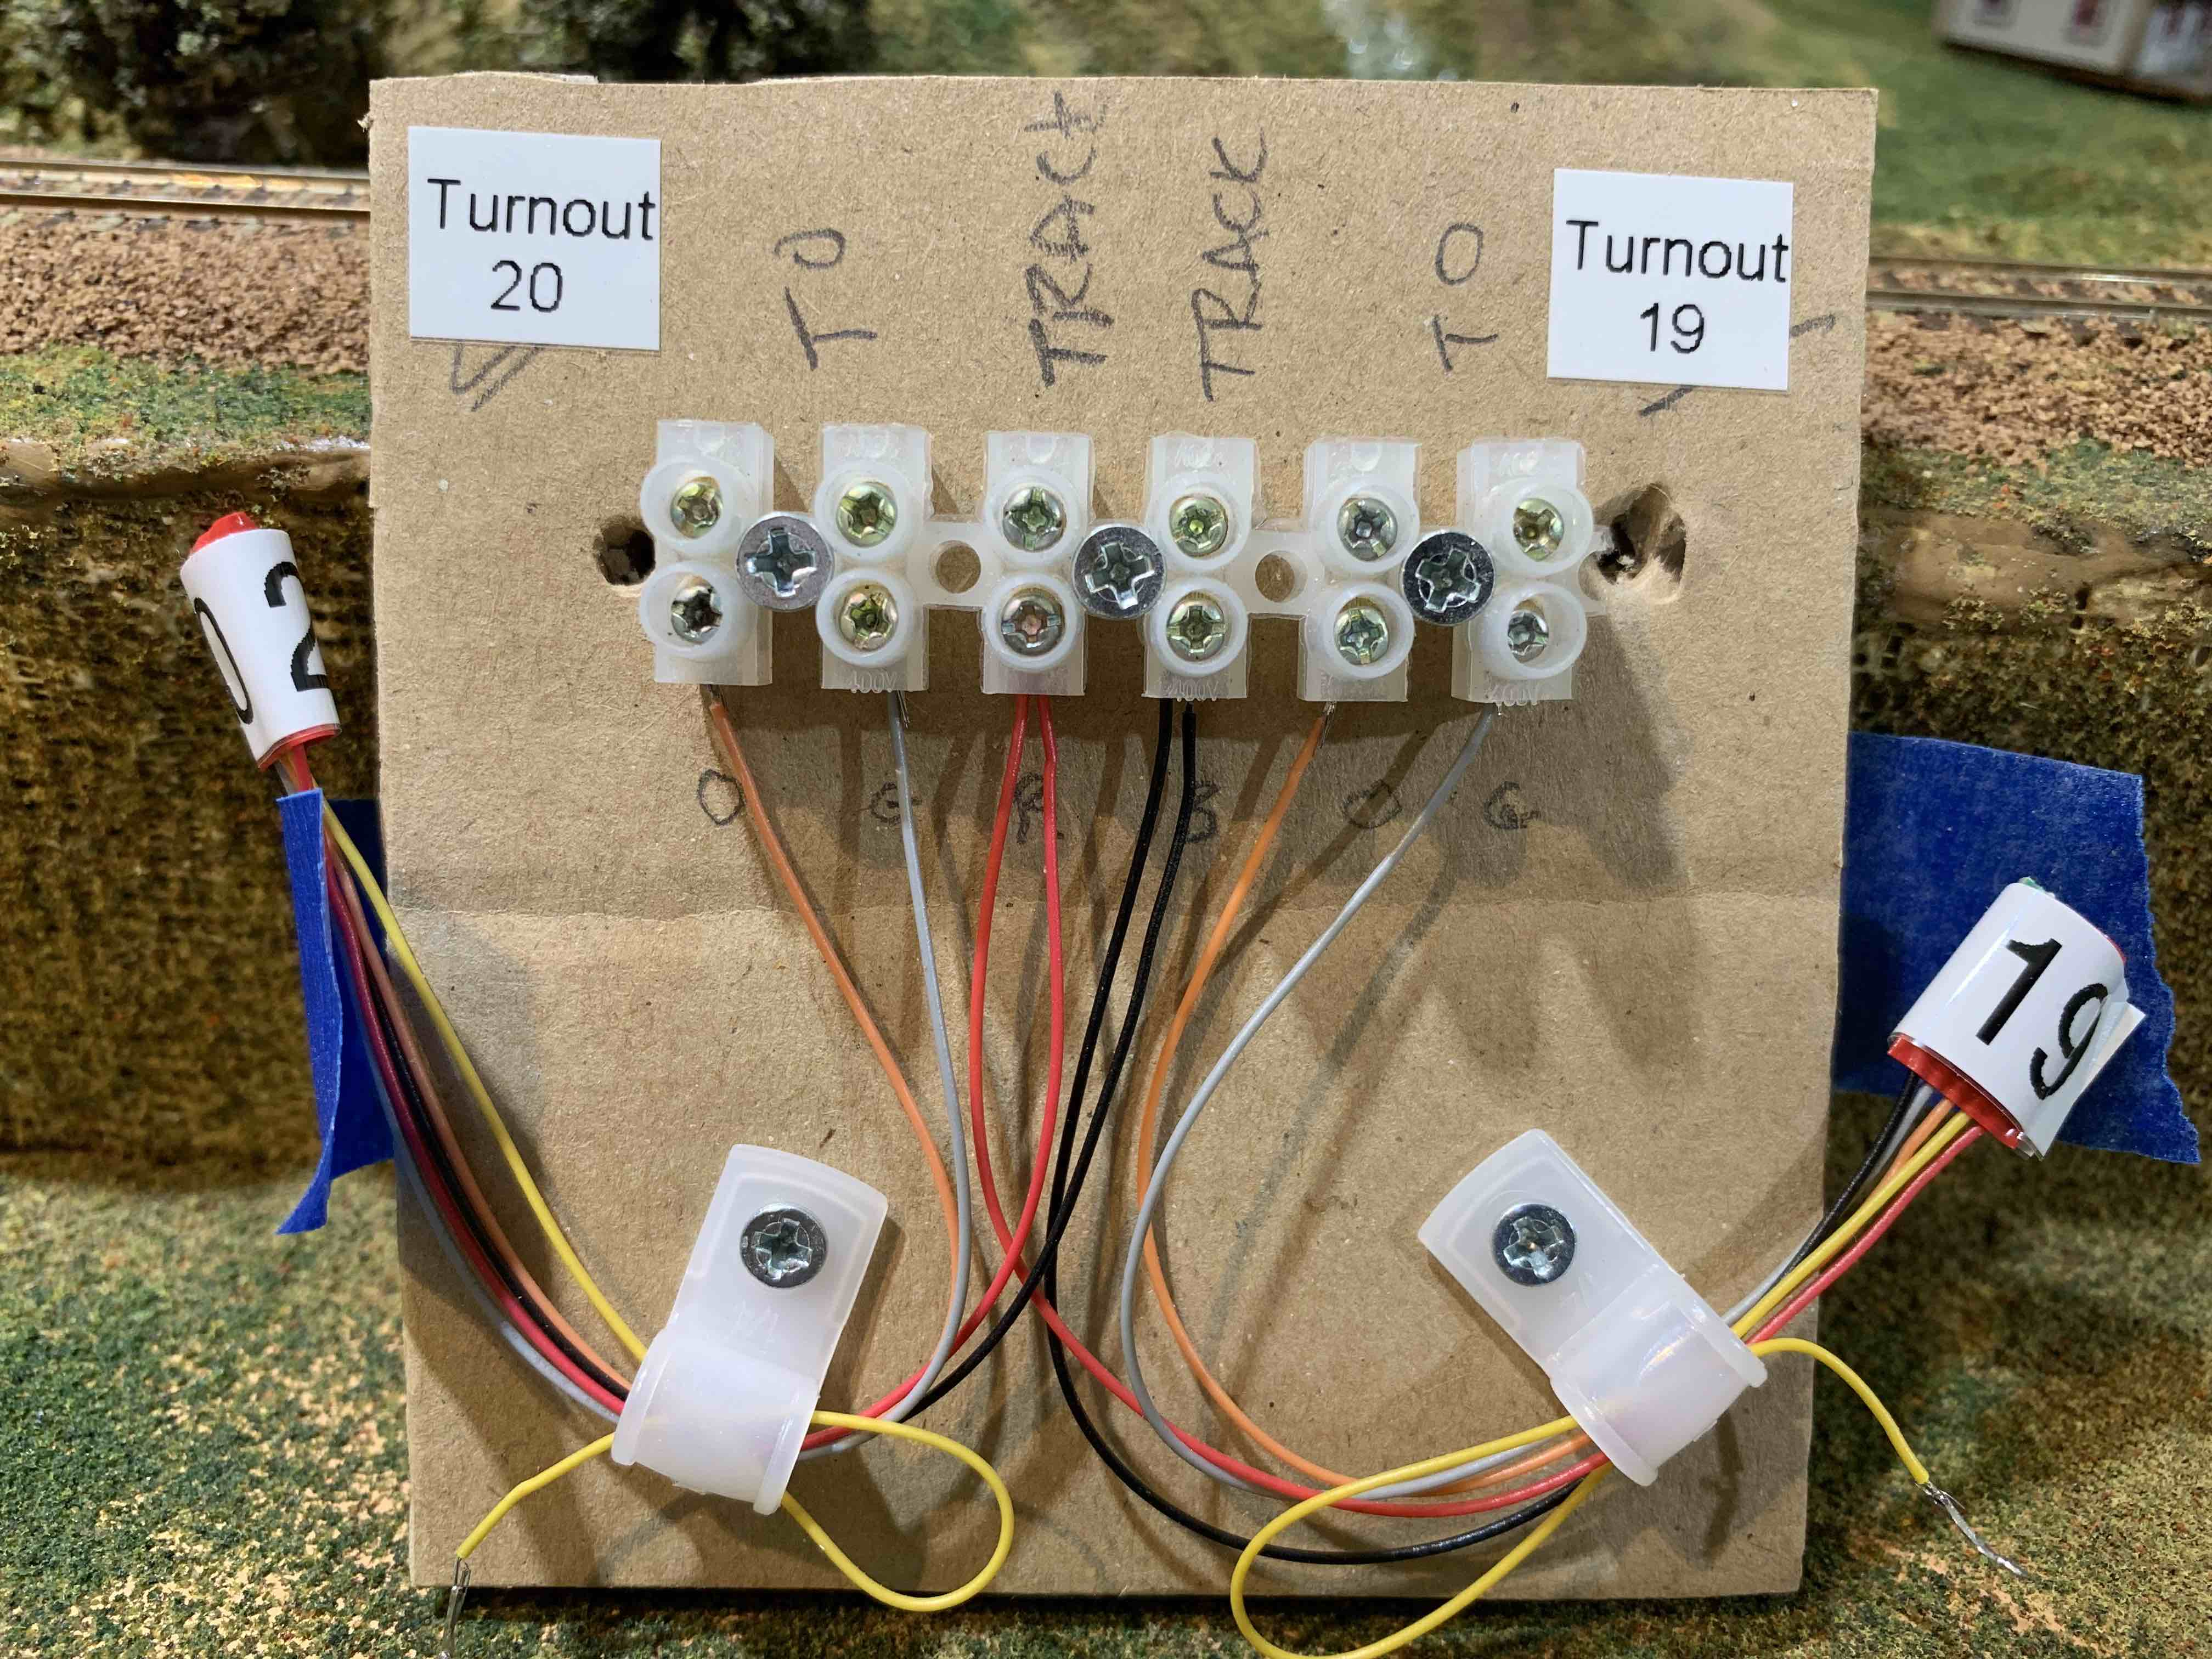
\includegraphics[width=0.4\textwidth]{./figures/printer/TwoNakedDecoders.jpg}
	\caption{Accessory decoders taped to underside of layout.}
	\label{fig:naked}
	\end{figure}
	
	\begin{figure}[htbp]
	\centering
	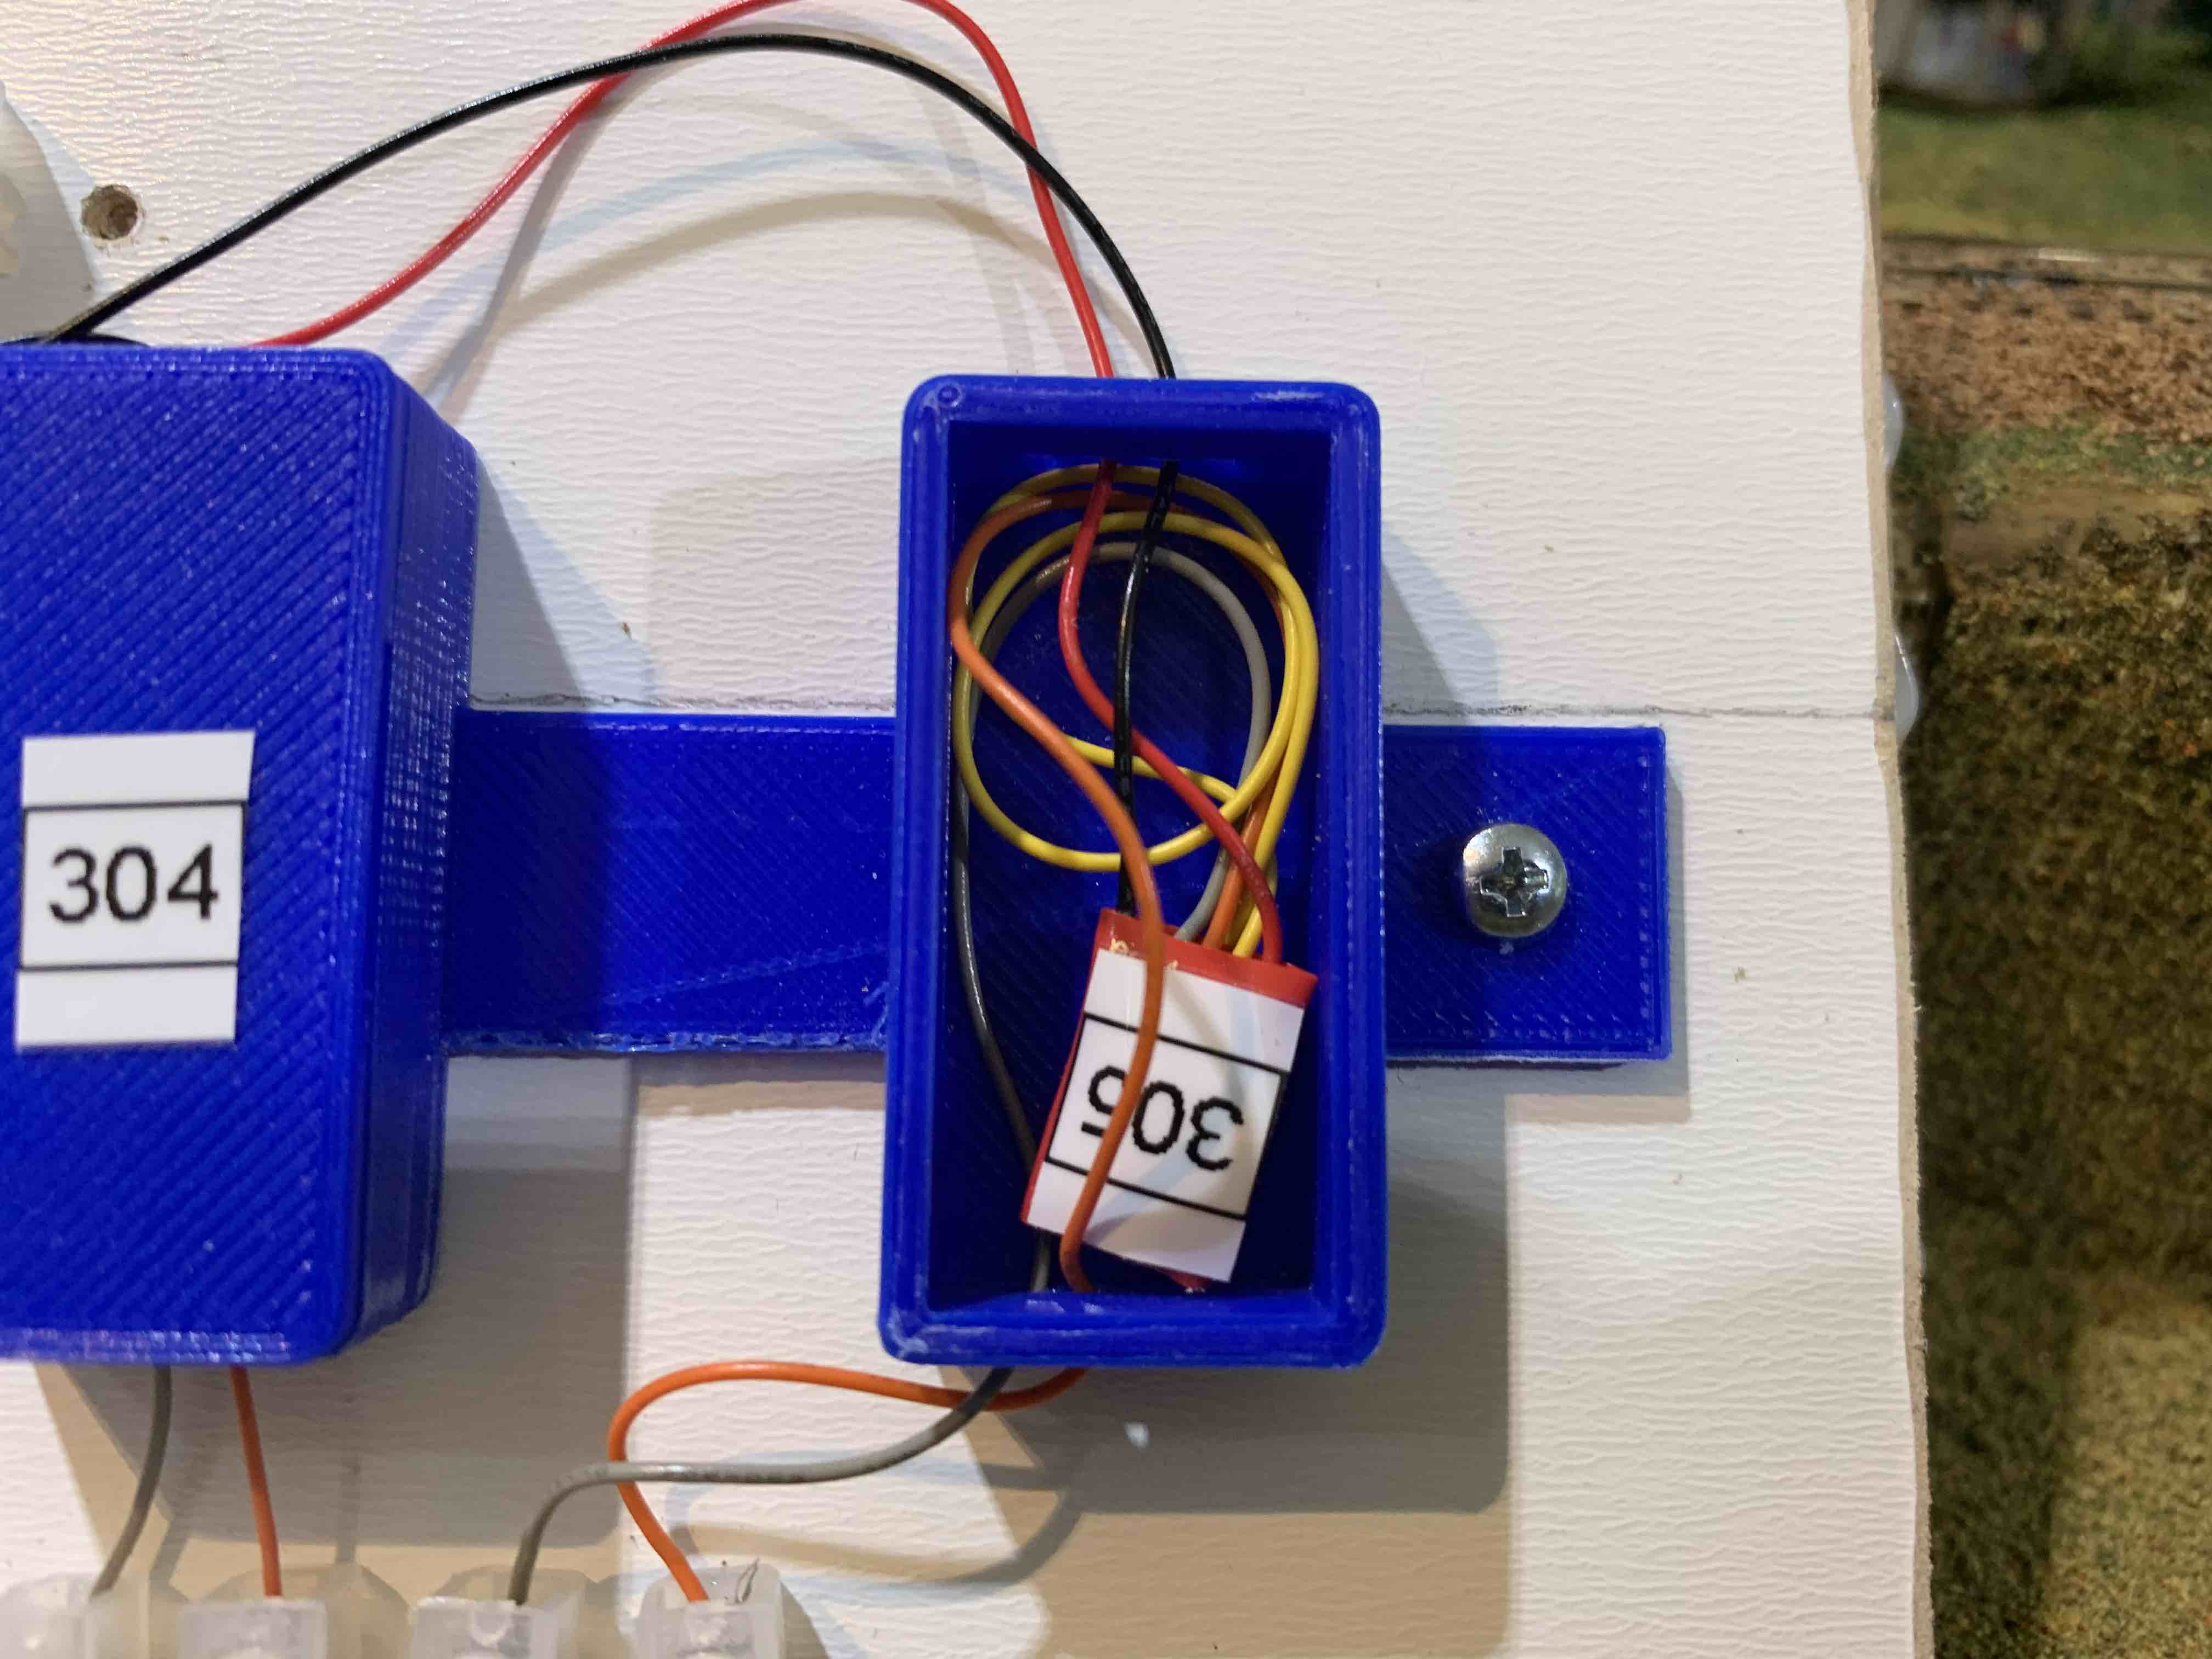
\includegraphics[width=0.4\textwidth]{./figures/printer/DecoderInBox.jpg}
	\caption{Decoder in 3D box, simplifying the appearance.}
		\label{fig:decoderInBox}
	\end{figure}
	
    \begin{figure}[htpb]
        \centering
        \begin{subfigure}[b]{0.475\textwidth}
            \centering
            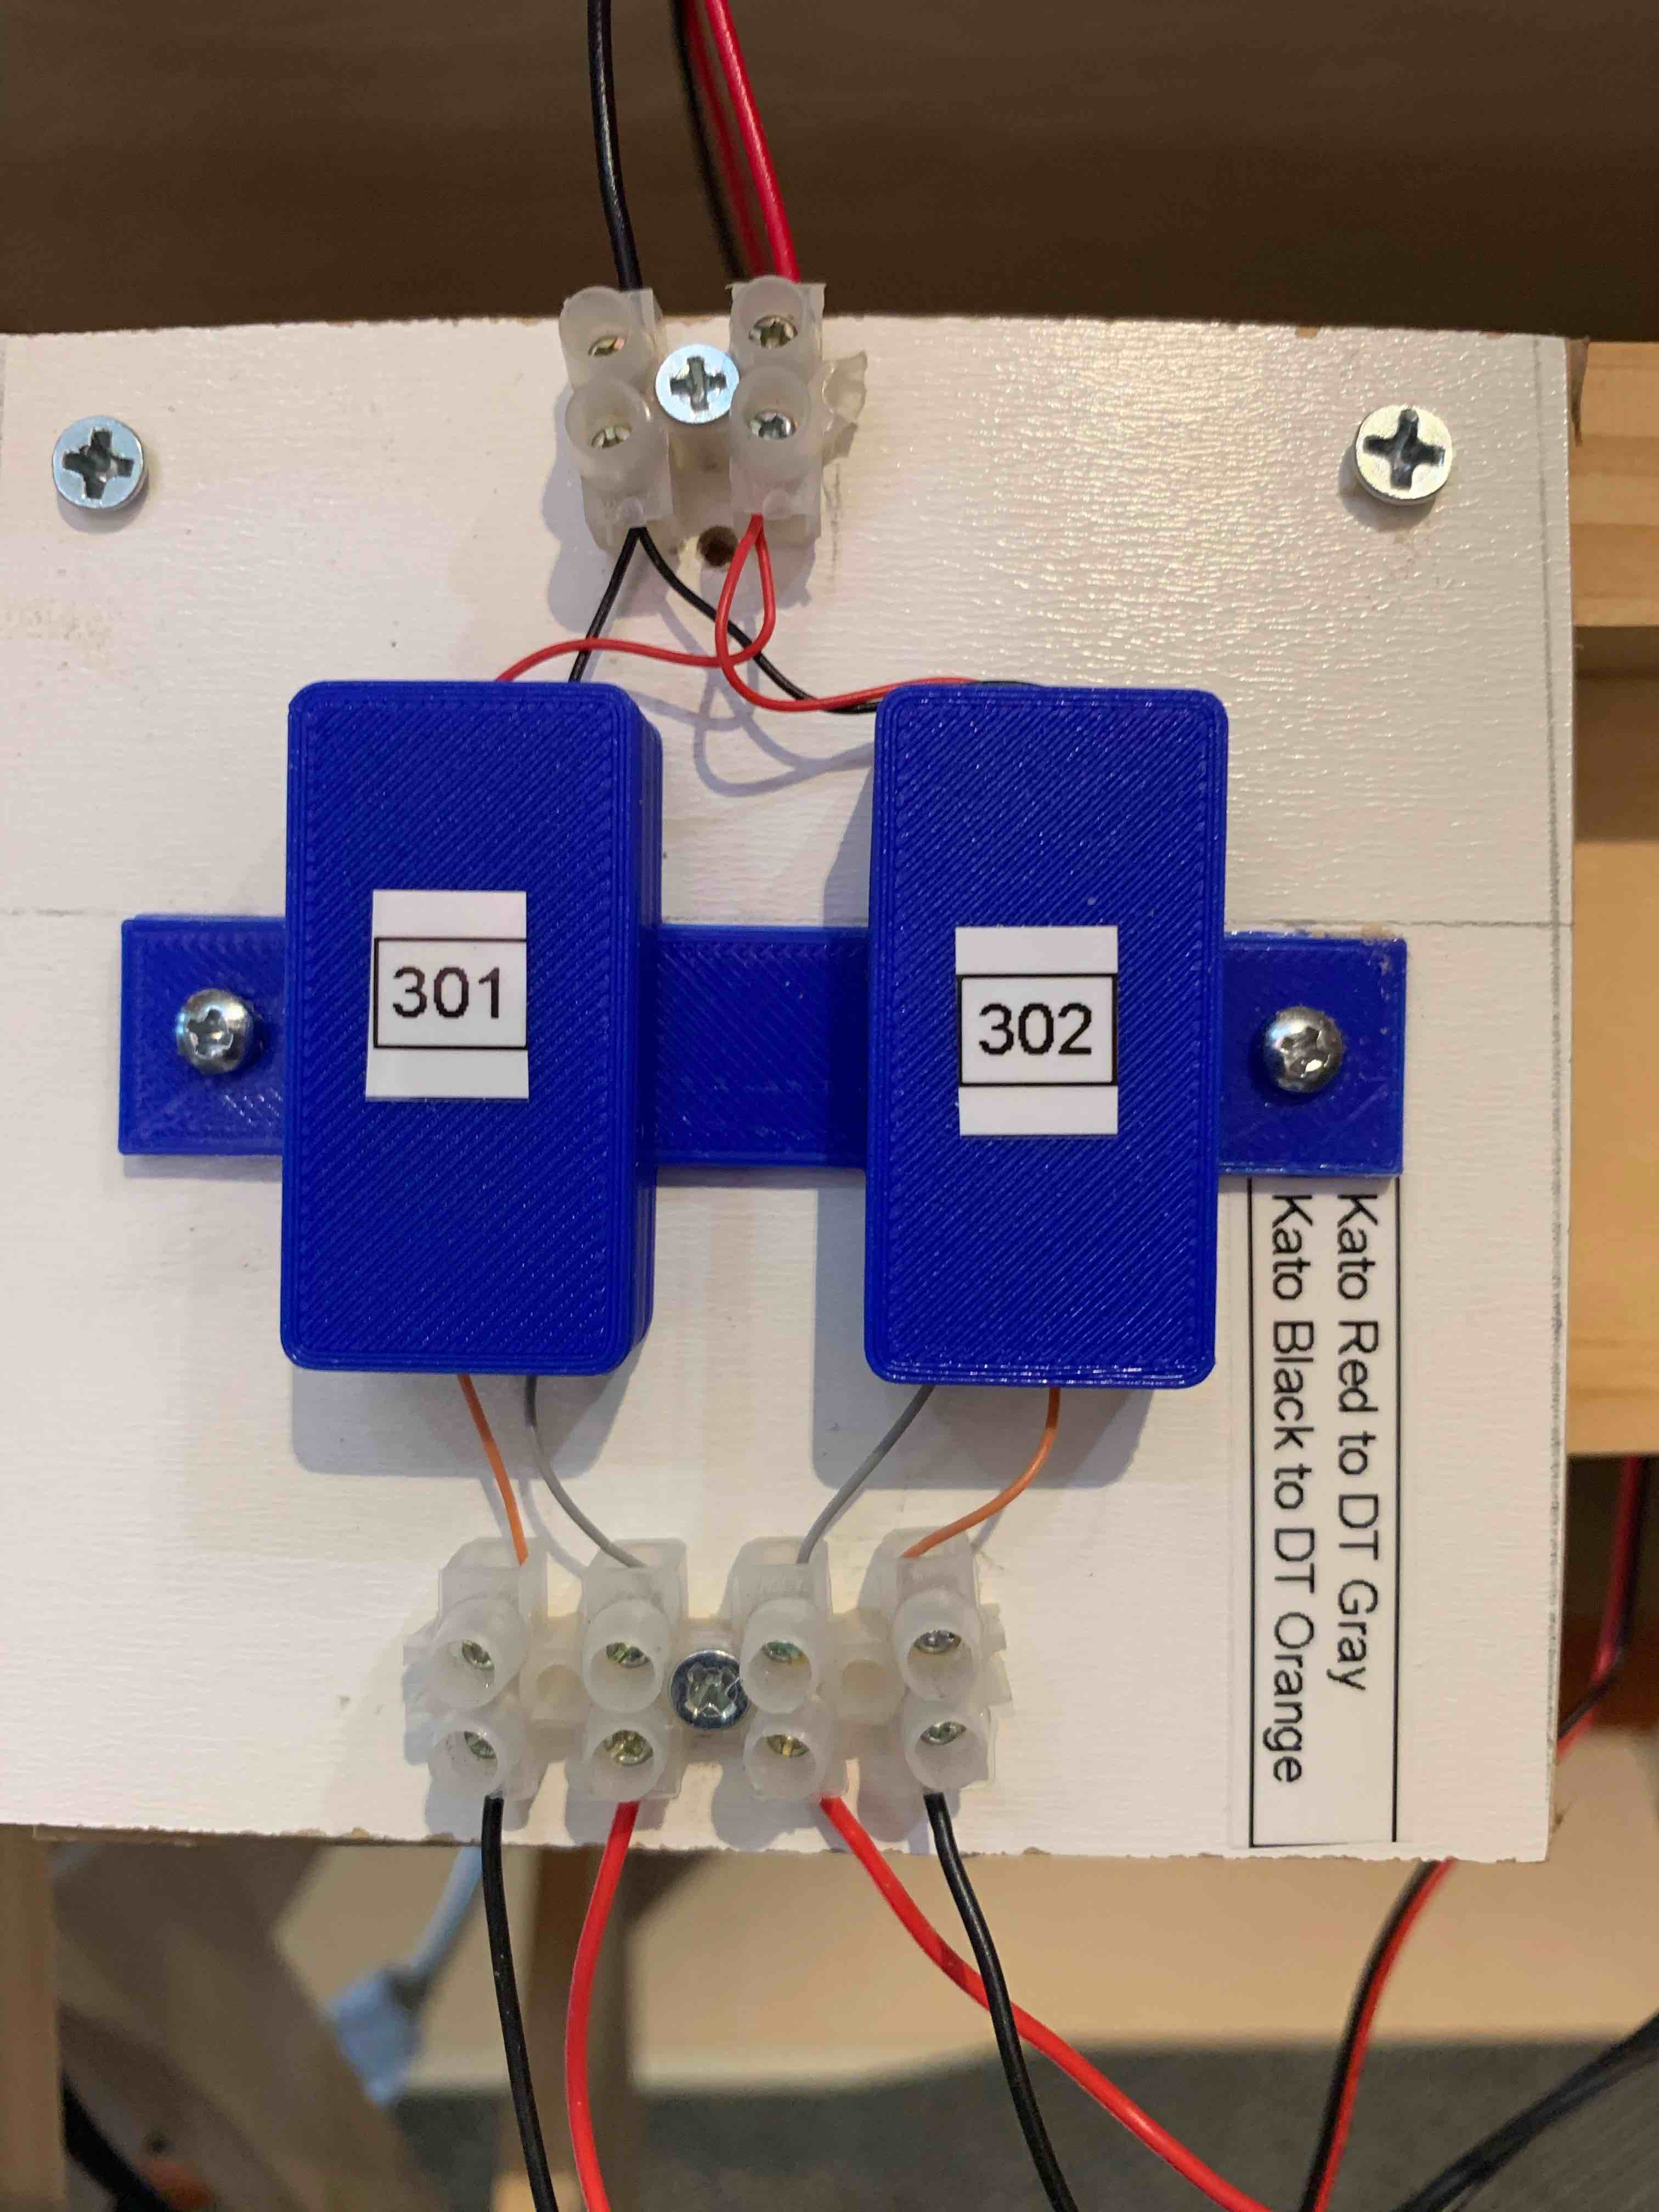
\includegraphics[width=\textwidth]{./figures/printer/TwoBoxes.jpg}
           \caption{Print of two boxes}
        \end{subfigure}
        \hfill
        \begin{subfigure}[b]{0.475\textwidth}
            \centering 
            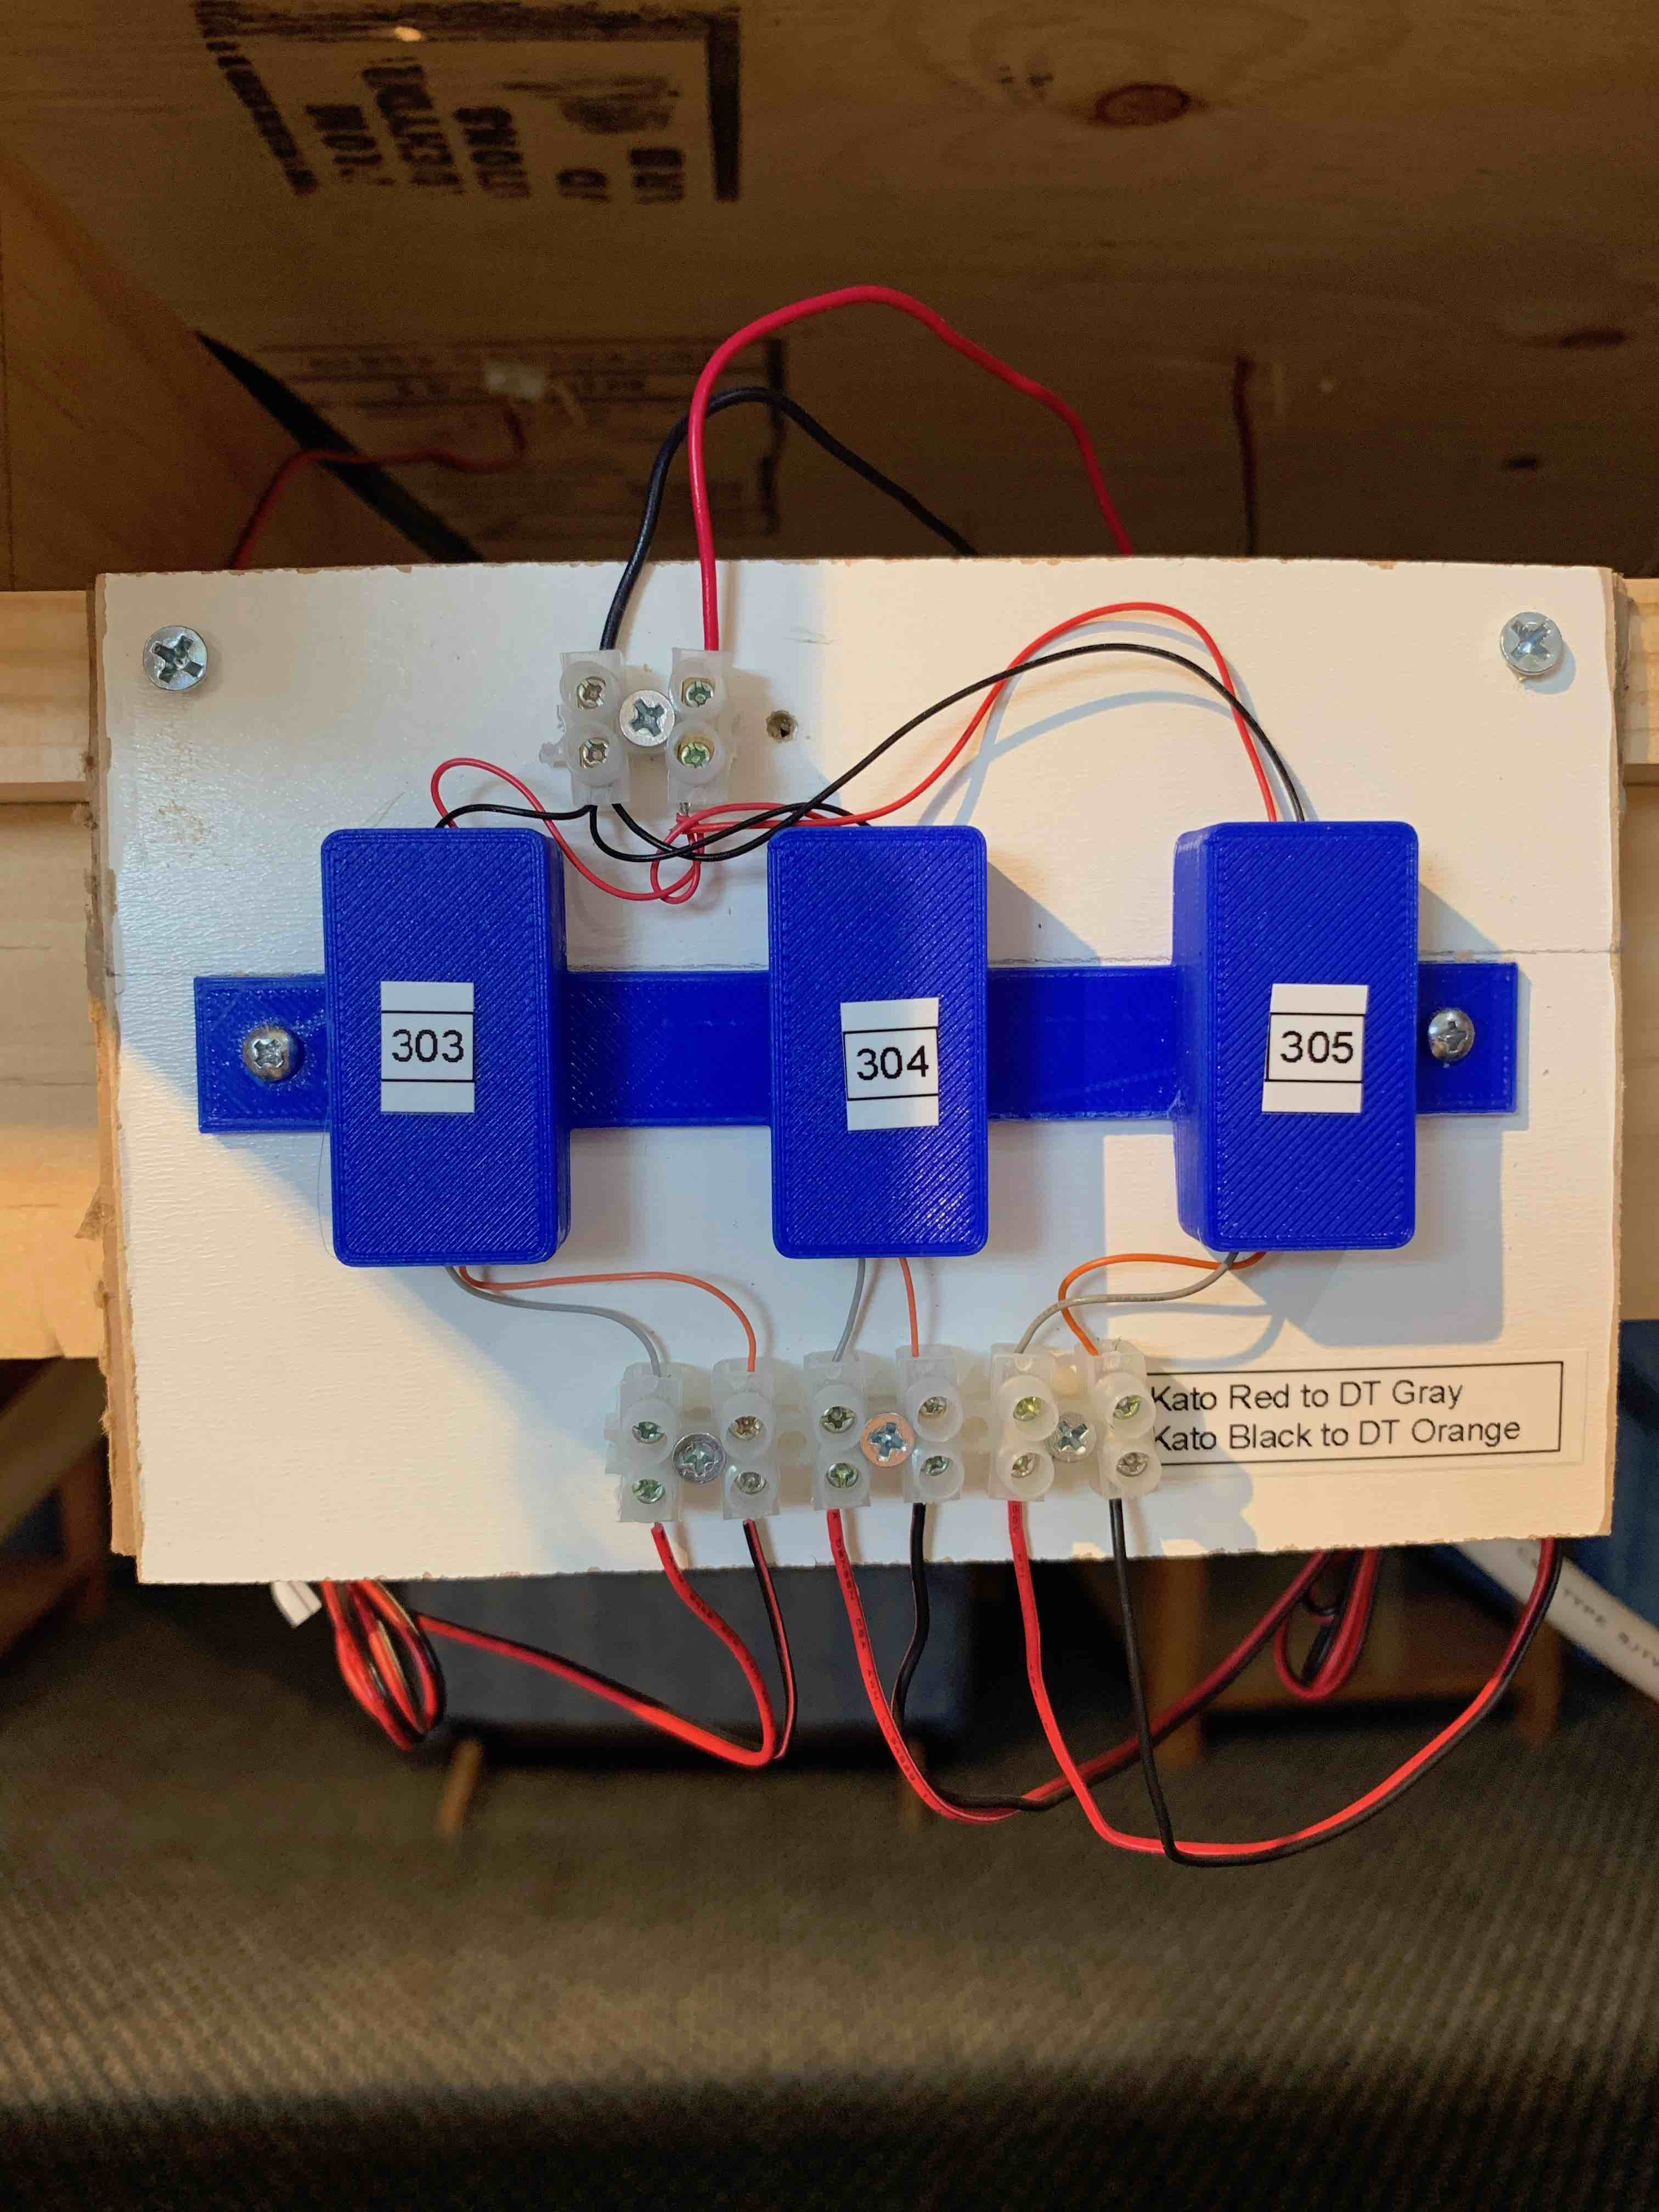
\includegraphics[width=\textwidth]{./figures/printer/ThreeBoxes.jpg}
           \caption{Print of three boxes}
        \end{subfigure}
        \vskip\baselineskip
        \begin{subfigure}[b] {0.475\textwidth}
            \centering 
            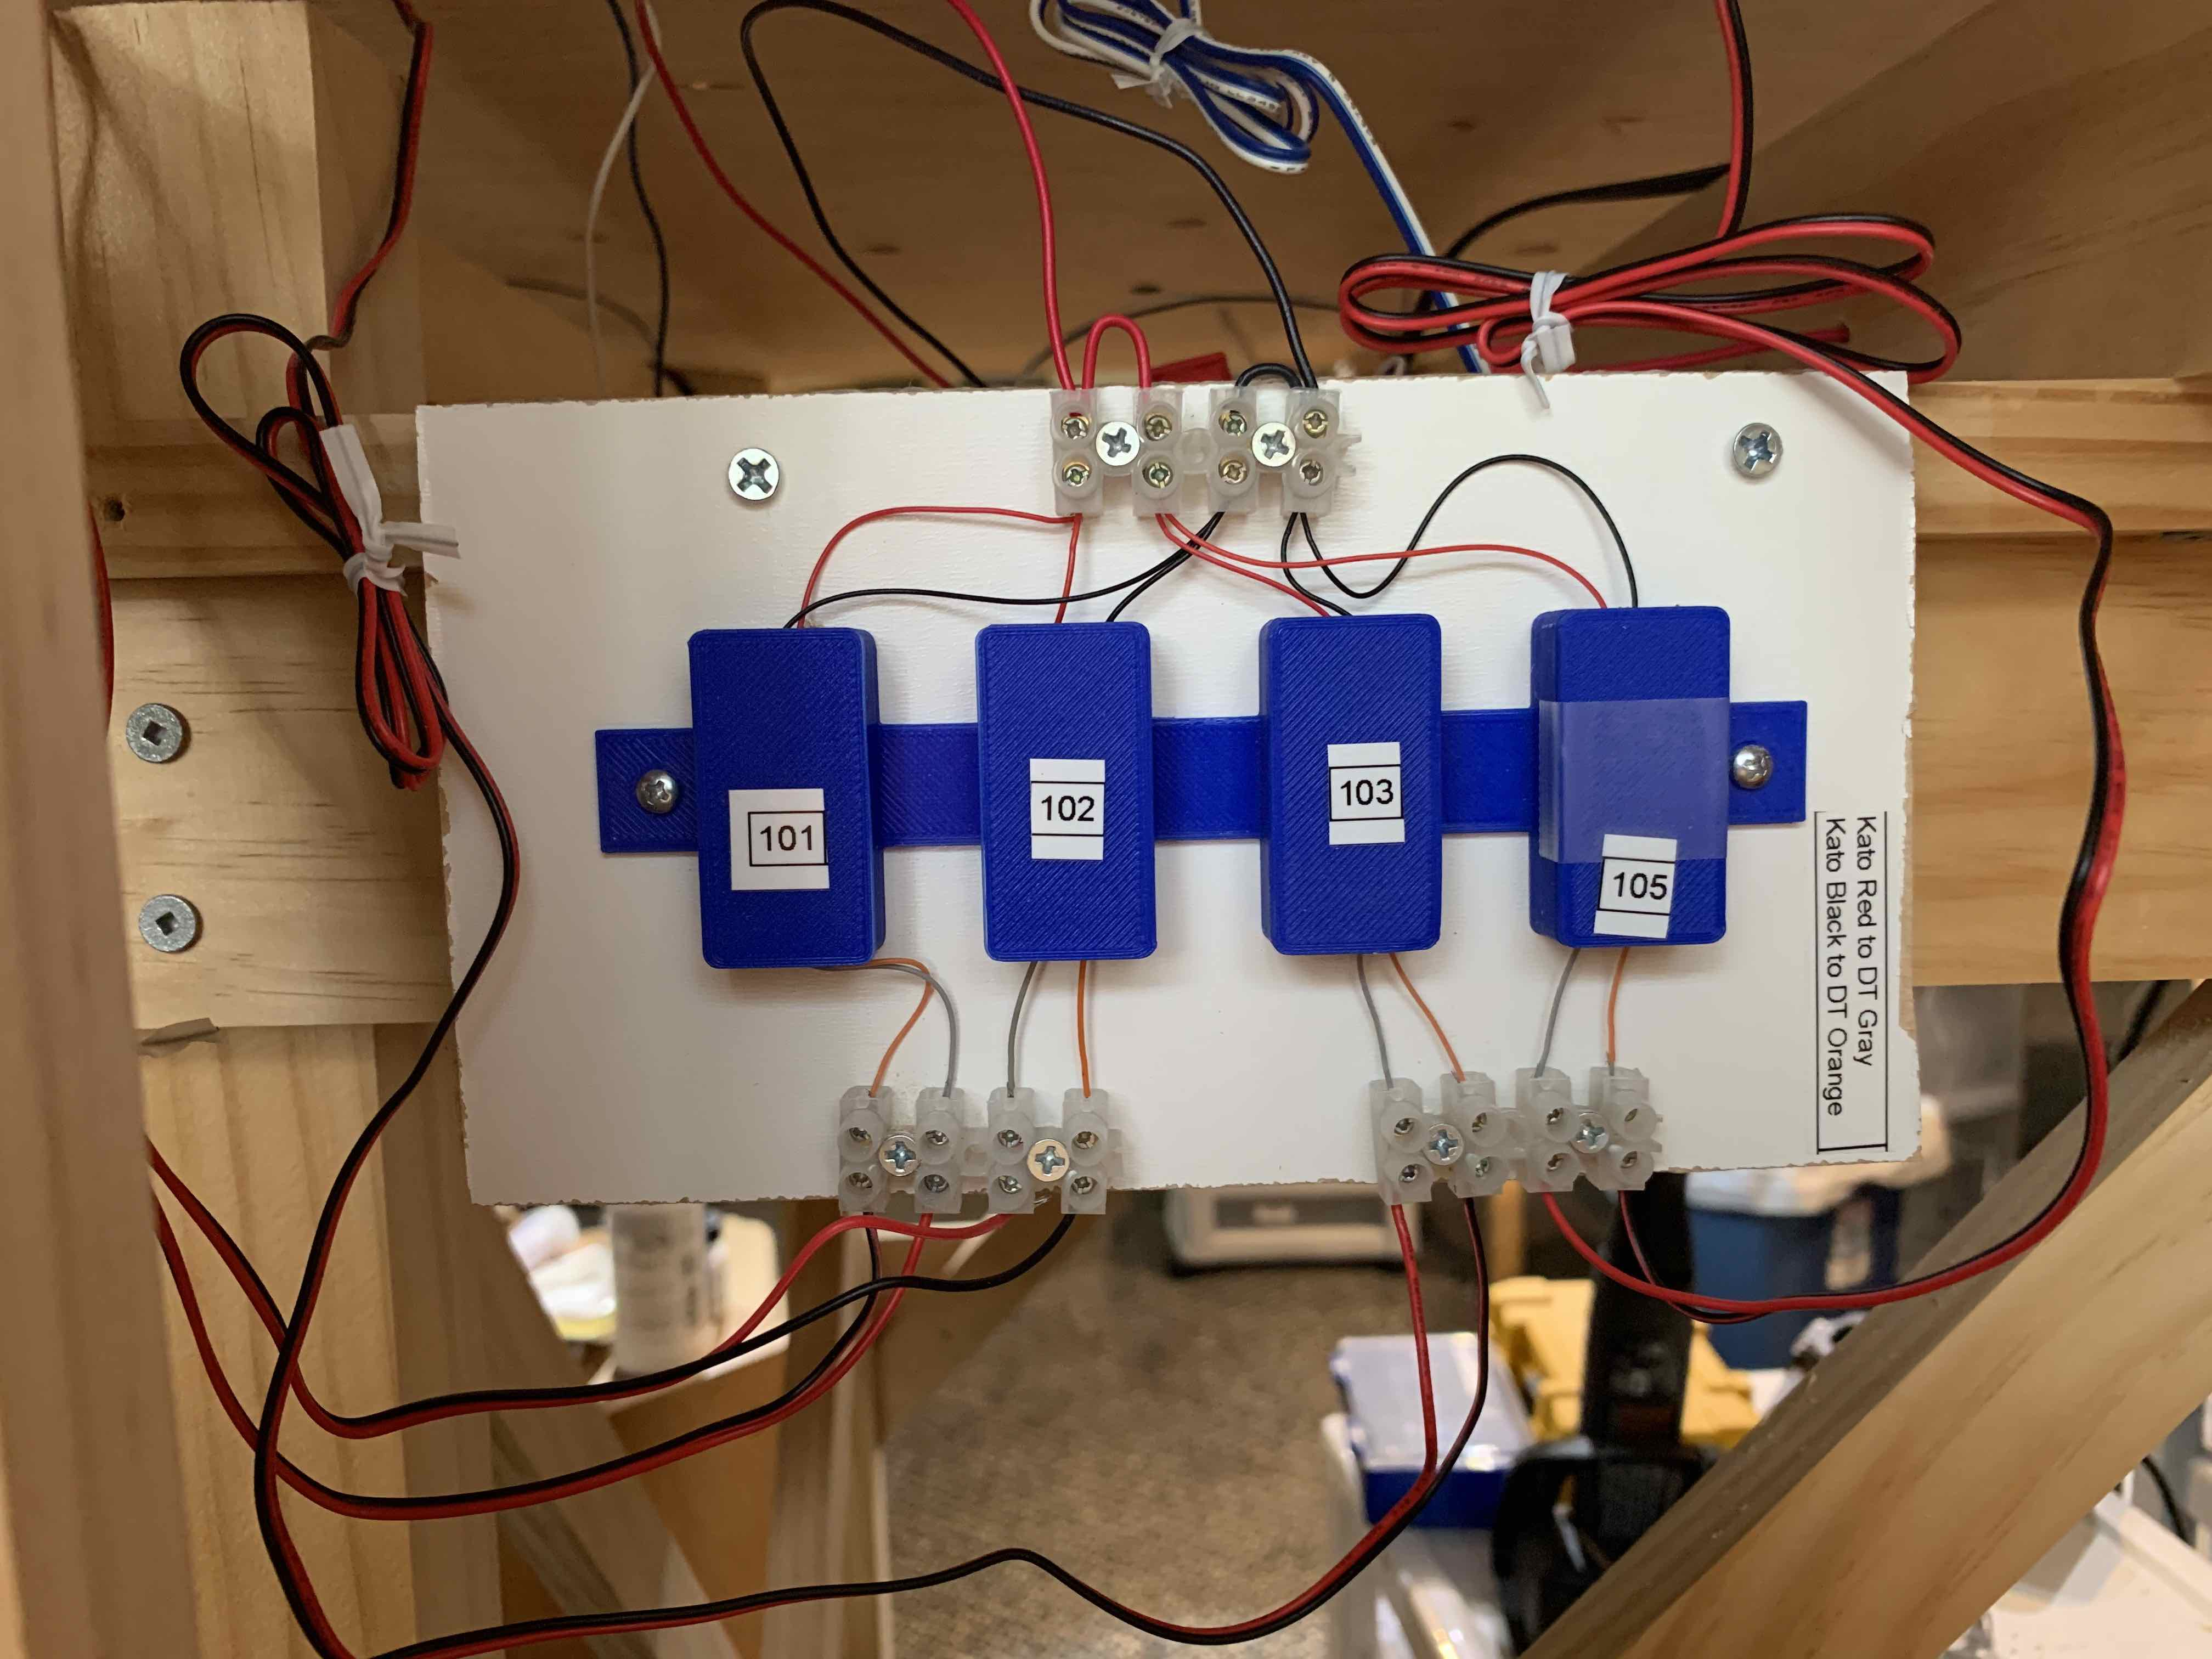
\includegraphics[width=\textwidth]{./figures/printer/FourBoxes.jpg}
         \caption{Print of four boxes}
        \end{subfigure}
        \quad
        \begin{subfigure}[b]  {0.475\textwidth}
            \centering 
            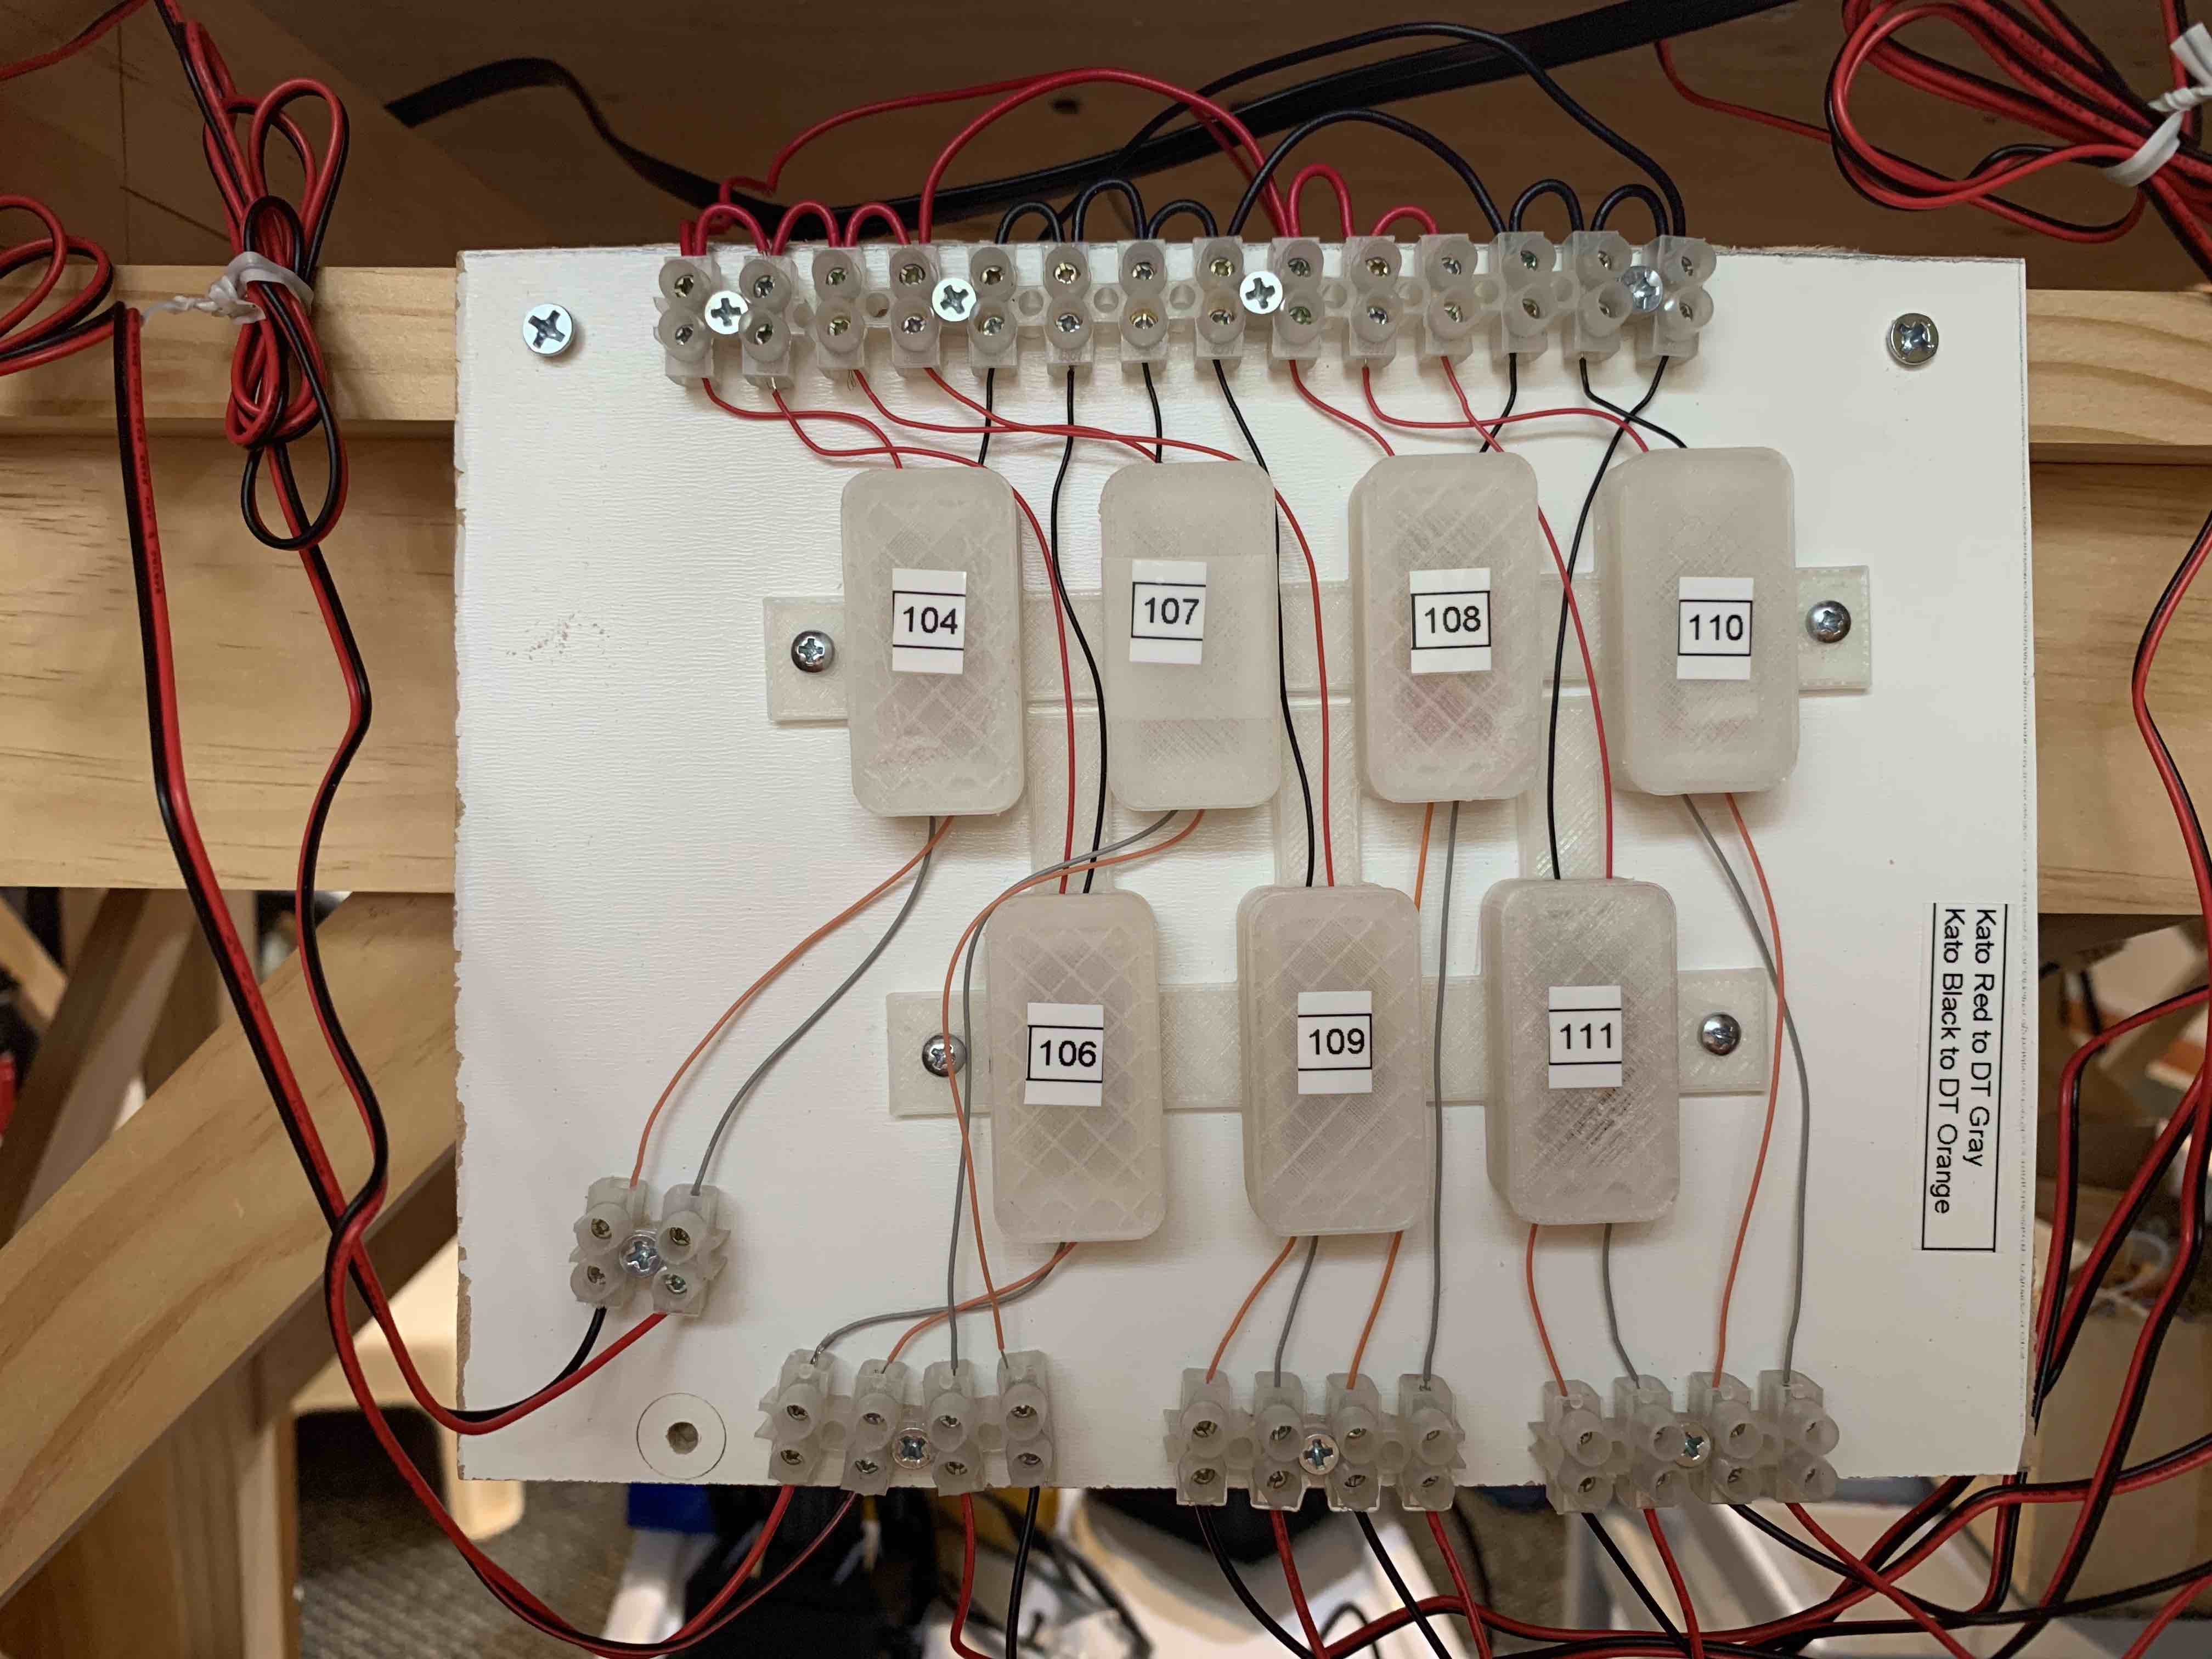
\includegraphics[width=\textwidth]{./figures/printer/SevenBoxes.jpg}
          \caption{Print of seven boxes}
        \end{subfigure}
        \caption {3D assorted size printed boxes to contain accessory decoders for Kato turnouts.} 
        \label{fig:decoderBoxes}
    \end{figure}
    
\section{Printing Structures and Rolling Stock}
To be written.

\part{Test Track}
% This document contains site monitoring information for the relevant network
%
%  				J. Michael Dean, M.D.
%  				University of Utah School of Medicine

% The following line makes this document point back so that my software will synchronize
% between the preview and source windows.

%!TEX root = ../Railroad.tex

\chapter{Test Chapter}
\minitoc
\index{test}


The primary responsibility of the Data and Safety Monitoring Board (DSMB) is to ensure the safety of the patients.
\begin{itemize}
	\item The DSMB will be composed of a minimum of three clinicians who have experience in clinical studies  and one biostatistician with experience in the monitoring and analysis of clinical trials.  None of the members will be investigators in the study.
	\item The proceedings of each DSMB meeting, whether held face-to-face or as a teleconference, will be recorded in minutes.  Copies of the minutes will be maintained by the Secretary of the DSMB, archived and kept confidential.  Access to the minutes by the sponsor or study investigators will be prohibited until after the trial database has been locked and the study has been unblinded.
\end{itemize}

The primary responsibility of the Data and Safety Monitoring Board (DSMB) is to ensure the safety of the patients.
\begin{itemize}
	\item The DSMB will be composed of a minimum of three clinicians who have experience in clinical studies  and one biostatistician with experience in the monitoring and analysis of clinical trials.  None of the members will be investigators in the study.
	\item The proceedings of each DSMB meeting, whether held face-to-face or as a teleconference, will be recorded in minutes.  Copies of the minutes will be maintained by the Secretary of the DSMB, archived and kept confidential.  Access to the minutes by the sponsor or study investigators will be prohibited until after the trial database has been locked and the study has been unblinded.
\end{itemize}

The primary responsibility of the Data and Safety Monitoring Board (DSMB) is to ensure the safety of the patients.
\begin{itemize}
	\item The DSMB will be composed of a minimum of three clinicians who have experience in clinical studies  and one biostatistician with experience in the monitoring and analysis of clinical trials.  None of the members will be investigators in the study.
	\item The proceedings of each DSMB meeting, whether held face-to-face or as a teleconference, will be recorded in minutes.  Copies of the minutes will be maintained by the Secretary of the DSMB, archived and kept confidential.  Access to the minutes by the sponsor or study investigators will be prohibited until after the trial database has been locked and the study has been unblinded.
\end{itemize}

The primary responsibility of the Data and Safety Monitoring Board (DSMB) is to ensure the safety of the patients.
\begin{itemize}
	\item The DSMB will be composed of a minimum of three clinicians who have experience in clinical studies  and one biostatistician with experience in the monitoring and analysis of clinical trials.  None of the members will be investigators in the study.
	\item The proceedings of each DSMB meeting, whether held face-to-face or as a teleconference, will be recorded in minutes.  Copies of the minutes will be maintained by the Secretary of the DSMB, archived and kept confidential.  Access to the minutes by the sponsor or study investigators will be prohibited until after the trial database has been locked and the study has been unblinded.
\end{itemize}

The primary responsibility of the Data and Safety Monitoring Board (DSMB) is to ensure the safety of the patients.
\begin{itemize}
	\item The DSMB will be composed of a minimum of three clinicians who have experience in clinical studies  and one biostatistician with experience in the monitoring and analysis of clinical trials.  None of the members will be investigators in the study.
	\item The proceedings of each DSMB meeting, whether held face-to-face or as a teleconference, will be recorded in minutes.  Copies of the minutes will be maintained by the Secretary of the DSMB, archived and kept confidential.  Access to the minutes by the sponsor or study investigators will be prohibited until after the trial database has been locked and the study has been unblinded.
\end{itemize}

The primary responsibility of the Data and Safety Monitoring Board (DSMB) is to ensure the safety of the patients.
\begin{itemize}
	\item The DSMB will be composed of a minimum of three clinicians who have experience in clinical studies  and one biostatistician with experience in the monitoring and analysis of clinical trials.  None of the members will be investigators in the study.
	\item The proceedings of each DSMB meeting, whether held face-to-face or as a teleconference, will be recorded in minutes.  Copies of the minutes will be maintained by the Secretary of the DSMB, archived and kept confidential.  Access to the minutes by the sponsor or study investigators will be prohibited until after the trial database has been locked and the study has been unblinded.
\end{itemize}

The primary responsibility of the Data and Safety Monitoring Board (DSMB) is to ensure the safety of the patients.
\begin{itemize}
	\item The DSMB will be composed of a minimum of three clinicians who have experience in clinical studies  and one biostatistician with experience in the monitoring and analysis of clinical trials.  None of the members will be investigators in the study.
	\item The proceedings of each DSMB meeting, whether held face-to-face or as a teleconference, will be recorded in minutes.  Copies of the minutes will be maintained by the Secretary of the DSMB, archived and kept confidential.  Access to the minutes by the sponsor or study investigators will be prohibited until after the trial database has been locked and the study has been unblinded.
\end{itemize}

The primary responsibility of the Data and Safety Monitoring Board (DSMB) is to ensure the safety of the patients.
\begin{itemize}
	\item The DSMB will be composed of a minimum of three clinicians who have experience in clinical studies  and one biostatistician with experience in the monitoring and analysis of clinical trials.  None of the members will be investigators in the study.
	\item The proceedings of each DSMB meeting, whether held face-to-face or as a teleconference, will be recorded in minutes.  Copies of the minutes will be maintained by the Secretary of the DSMB, archived and kept confidential.  Access to the minutes by the sponsor or study investigators will be prohibited until after the trial database has been locked and the study has been unblinded.
\end{itemize}

The primary responsibility of the Data and Safety Monitoring Board (DSMB) is to ensure the safety of the patients.
\begin{itemize}
	\item The DSMB will be composed of a minimum of three clinicians who have experience in clinical studies  and one biostatistician with experience in the monitoring and analysis of clinical trials.  None of the members will be investigators in the study.
	\item The proceedings of each DSMB meeting, whether held face-to-face or as a teleconference, will be recorded in minutes.  Copies of the minutes will be maintained by the Secretary of the DSMB, archived and kept confidential.  Access to the minutes by the sponsor or study investigators will be prohibited until after the trial database has been locked and the study has been unblinded.
\end{itemize}

The primary responsibility of the Data and Safety Monitoring Board (DSMB) is to ensure the safety of the patients.
\begin{itemize}
	\item The DSMB will be composed of a minimum of three clinicians who have experience in clinical studies  and one biostatistician with experience in the monitoring and analysis of clinical trials.  None of the members will be investigators in the study.
	\item The proceedings of each DSMB meeting, whether held face-to-face or as a teleconference, will be recorded in minutes.  Copies of the minutes will be maintained by the Secretary of the DSMB, archived and kept confidential.  Access to the minutes by the sponsor or study investigators will be prohibited until after the trial database has been locked and the study has been unblinded.
\end{itemize}

\part{Electronics}
% This document contains site monitoring information for the relevant network
%
%  				J. Michael Dean, M.D.
%  				University of Utah School of Medicine

% The following line makes this document point back so that my software will synchronize
% between the preview and source windows.

%!TEX root = ../Railroad.tex

\chapter{Test Chapter}
\minitoc
\index{test}


The primary responsibility of the Data and Safety Monitoring Board (DSMB) is to ensure the safety of the patients.
\begin{itemize}
	\item The DSMB will be composed of a minimum of three clinicians who have experience in clinical studies  and one biostatistician with experience in the monitoring and analysis of clinical trials.  None of the members will be investigators in the study.
	\item The proceedings of each DSMB meeting, whether held face-to-face or as a teleconference, will be recorded in minutes.  Copies of the minutes will be maintained by the Secretary of the DSMB, archived and kept confidential.  Access to the minutes by the sponsor or study investigators will be prohibited until after the trial database has been locked and the study has been unblinded.
\end{itemize}

The primary responsibility of the Data and Safety Monitoring Board (DSMB) is to ensure the safety of the patients.
\begin{itemize}
	\item The DSMB will be composed of a minimum of three clinicians who have experience in clinical studies  and one biostatistician with experience in the monitoring and analysis of clinical trials.  None of the members will be investigators in the study.
	\item The proceedings of each DSMB meeting, whether held face-to-face or as a teleconference, will be recorded in minutes.  Copies of the minutes will be maintained by the Secretary of the DSMB, archived and kept confidential.  Access to the minutes by the sponsor or study investigators will be prohibited until after the trial database has been locked and the study has been unblinded.
\end{itemize}

The primary responsibility of the Data and Safety Monitoring Board (DSMB) is to ensure the safety of the patients.
\begin{itemize}
	\item The DSMB will be composed of a minimum of three clinicians who have experience in clinical studies  and one biostatistician with experience in the monitoring and analysis of clinical trials.  None of the members will be investigators in the study.
	\item The proceedings of each DSMB meeting, whether held face-to-face or as a teleconference, will be recorded in minutes.  Copies of the minutes will be maintained by the Secretary of the DSMB, archived and kept confidential.  Access to the minutes by the sponsor or study investigators will be prohibited until after the trial database has been locked and the study has been unblinded.
\end{itemize}

The primary responsibility of the Data and Safety Monitoring Board (DSMB) is to ensure the safety of the patients.
\begin{itemize}
	\item The DSMB will be composed of a minimum of three clinicians who have experience in clinical studies  and one biostatistician with experience in the monitoring and analysis of clinical trials.  None of the members will be investigators in the study.
	\item The proceedings of each DSMB meeting, whether held face-to-face or as a teleconference, will be recorded in minutes.  Copies of the minutes will be maintained by the Secretary of the DSMB, archived and kept confidential.  Access to the minutes by the sponsor or study investigators will be prohibited until after the trial database has been locked and the study has been unblinded.
\end{itemize}

The primary responsibility of the Data and Safety Monitoring Board (DSMB) is to ensure the safety of the patients.
\begin{itemize}
	\item The DSMB will be composed of a minimum of three clinicians who have experience in clinical studies  and one biostatistician with experience in the monitoring and analysis of clinical trials.  None of the members will be investigators in the study.
	\item The proceedings of each DSMB meeting, whether held face-to-face or as a teleconference, will be recorded in minutes.  Copies of the minutes will be maintained by the Secretary of the DSMB, archived and kept confidential.  Access to the minutes by the sponsor or study investigators will be prohibited until after the trial database has been locked and the study has been unblinded.
\end{itemize}

The primary responsibility of the Data and Safety Monitoring Board (DSMB) is to ensure the safety of the patients.
\begin{itemize}
	\item The DSMB will be composed of a minimum of three clinicians who have experience in clinical studies  and one biostatistician with experience in the monitoring and analysis of clinical trials.  None of the members will be investigators in the study.
	\item The proceedings of each DSMB meeting, whether held face-to-face or as a teleconference, will be recorded in minutes.  Copies of the minutes will be maintained by the Secretary of the DSMB, archived and kept confidential.  Access to the minutes by the sponsor or study investigators will be prohibited until after the trial database has been locked and the study has been unblinded.
\end{itemize}

The primary responsibility of the Data and Safety Monitoring Board (DSMB) is to ensure the safety of the patients.
\begin{itemize}
	\item The DSMB will be composed of a minimum of three clinicians who have experience in clinical studies  and one biostatistician with experience in the monitoring and analysis of clinical trials.  None of the members will be investigators in the study.
	\item The proceedings of each DSMB meeting, whether held face-to-face or as a teleconference, will be recorded in minutes.  Copies of the minutes will be maintained by the Secretary of the DSMB, archived and kept confidential.  Access to the minutes by the sponsor or study investigators will be prohibited until after the trial database has been locked and the study has been unblinded.
\end{itemize}

The primary responsibility of the Data and Safety Monitoring Board (DSMB) is to ensure the safety of the patients.
\begin{itemize}
	\item The DSMB will be composed of a minimum of three clinicians who have experience in clinical studies  and one biostatistician with experience in the monitoring and analysis of clinical trials.  None of the members will be investigators in the study.
	\item The proceedings of each DSMB meeting, whether held face-to-face or as a teleconference, will be recorded in minutes.  Copies of the minutes will be maintained by the Secretary of the DSMB, archived and kept confidential.  Access to the minutes by the sponsor or study investigators will be prohibited until after the trial database has been locked and the study has been unblinded.
\end{itemize}

The primary responsibility of the Data and Safety Monitoring Board (DSMB) is to ensure the safety of the patients.
\begin{itemize}
	\item The DSMB will be composed of a minimum of three clinicians who have experience in clinical studies  and one biostatistician with experience in the monitoring and analysis of clinical trials.  None of the members will be investigators in the study.
	\item The proceedings of each DSMB meeting, whether held face-to-face or as a teleconference, will be recorded in minutes.  Copies of the minutes will be maintained by the Secretary of the DSMB, archived and kept confidential.  Access to the minutes by the sponsor or study investigators will be prohibited until after the trial database has been locked and the study has been unblinded.
\end{itemize}

The primary responsibility of the Data and Safety Monitoring Board (DSMB) is to ensure the safety of the patients.
\begin{itemize}
	\item The DSMB will be composed of a minimum of three clinicians who have experience in clinical studies  and one biostatistician with experience in the monitoring and analysis of clinical trials.  None of the members will be investigators in the study.
	\item The proceedings of each DSMB meeting, whether held face-to-face or as a teleconference, will be recorded in minutes.  Copies of the minutes will be maintained by the Secretary of the DSMB, archived and kept confidential.  Access to the minutes by the sponsor or study investigators will be prohibited until after the trial database has been locked and the study has been unblinded.
\end{itemize}



%%%% Back matter of the book
\backmatter
\refstepcounter{chapter}
\addcontentsline{toc}{chapter}{Index}
\footnotesize
\printindex
\normalsize
\refstepcounter{chapter}

\end{document}
